\documentclass[journal]{IEEEtran}
\usepackage{amsmath,amsfonts}
%\usepackage{algorithmic}
\usepackage{algorithm}
\usepackage{array}
\usepackage[caption=false,font=scriptsize,labelfont=sf,textfont=sf]{subfig}
\usepackage{textcomp}
\usepackage{stfloats}
\usepackage{url}
\usepackage{verbatim}
\usepackage{graphicx}
\usepackage{cite}

\usepackage{multirow}
\usepackage{authblk}
\usepackage{booktabs}
\usepackage{algorithmicx}  
\usepackage{algpseudocode}
\usepackage{soul}
\hyphenation{op-tical net-works semi-conduc-tor IEEE-Xplore}
% updated with editorial comments 8/9/2021

\begin{document}

\title{Defending Byzantine Attacks in Ensemble Federated Learning: A Reputation-based Phishing Approach}
\author{Beibei~Li,~\IEEEmembership{Member,~IEEE,}
        Peiran~Wang,~\IEEEmembership{Student Member,~IEEE,}
        Qinglei~Kong,~\IEEEmembership{Member,~IEEE,}
        Yuan~Zhang,~\IEEEmembership{Member,~IEEE,}
        and~Rongxing~Lu,~\IEEEmembership{Fellow,~IEEE}
\thanks{This paper is an extended version of the paper titled `FLPhish: Reputation-Based Phishing Byzantine Defense in Ensemble Federated Learning', which was published in IEEE ISCC 2021, and awarded `Best Paper'.}
\thanks{B. Li and P. Wang are with the School of Cyber Science and Engineering, Sichuan Universsity, Chengdu, Sichuan, China 610065. Email: libeibei@scu.edu.cn; wangpeiran@stu.scu.edu.cn.}
\thanks{Q. Kong is with the Future Network of Intelligence Institute, The Chinese University of Hong Kong, Shenzhen, China 518172, and also with The University of Science and Technology of China, Hefei, China 230052. Email: kql8904@163.com.}
\thanks{Y. Zhang is with the School of Computer Science and Engineering, University of Electronic Science and Technology of China, Chengdu, China 610054. Email: zy\_loye@126.com.}
\thanks{R. Lu is with the Faculty of Computer Science, University of New Brunswick, Fredericton, NB, Canada E3B 5A3. Email: rlu1@unb.ca.}
}

% The paper headers
\markboth{IEEE TRANSACTIONS ON INFORMATION FORENSICS AND SECURITY}%
{Li \MakeLowercase{\textit{et al.}}: Defending Byzantine Attacks in Ensemble Federated Learning: A Reputation-based Phishing Approach}

%\IEEEpubid{0000--0000/00\$00.00~\copyright~2021 IEEE}
% Remember, if you use this you must call \IEEEpubidadjcol in the second
% column for its text to clear the IEEEpubid mark.

\maketitle

\begin{abstract}
  Emerging as a promising distributed learning paradigm, federated learning (FL) has been widely adopted in many fields. Nonetheless, a big challenge for FL in real-world implementation is Byzantine attacks, where compromised clients can mislead or poison the training model by falsifying or manipulating the local model parameters. To solve this problem, in this paper, we present a reputation-based Byzantine robust-FL scheme (called FLPhish) for defending Byzantine attacks under the Ensemble Federated Learning architecture (called EFL). Specifically, we first develop a novel ensemble FL architecture, EFL, which allows FL compatible with different deep learning models in different clients. Second, we craft a phishing algorithm for the EFL architecture to identify possible Byzantine behaviors. Third, a Bayesian inference based reputation mechanism is devised to measure each client's level of confidence and to further identify Byzantine clients. Last, we strictly analyze how the FLPhish scheme defend against backdoor attacks. Extensive experiments under different settings demonstrate that the proposed FLPhish achieves great efficacy in defending Byzantine attacks in EFL. FLPhish is tested with different fractions of Byzantine clients and different degrees of distribution imbalance.
\end{abstract}

\begin{IEEEkeywords}
  Federated learning, ensemble learning, Bayesian inference-based reputation, phishing.
\end{IEEEkeywords}

\begin{table}[t]
  \caption{Summary of Notations}
  \resizebox{0.5\textwidth}{!}{
  \begin{tabular}{lp{6cm}}
    \bottomrule
    Term&Description\\
    \hline
    $s$ & central server in FL \\
    $c_i$ & the $i$th client in FL, $i=1,2,3,...,u$ \\
    $d_i$ & the local dataset preserved by the $i$th client \\
    $C$ & the ensemble of all the clients \\
    $u$ & the number of clients\\
    $D_t$ & the unlabeled dataset chosen by $s$ in each procedure\\
    $D$ & the unlabeled dataset preserved by $s$\\
    $n$ & the number of samples in $D_t$\\
    $B_t$ & the labeled dataset (\textit{`bait'}) chosen by $s$ in each procedure\\
    $B$ & the labeled dataset preserved by $s$\\
    $m$ & the number of samples in $B_t$\\
    $a_i^t$ & the accuracy of predictions of $B_t$ made by $c_i$ in $t$th procedure\\
    $q_i$ & the label of $c_i$ to judge it is a malicious client or not\\
    $r_q$ & the threhold of malicious clients\\
    $x^t_l$ & the $l$th data point in $D_t$\\
    $b_i$ & the Byzantine attacker\\
    $\sigma$ & the `trigger' in the backdoor attack\\
    $\iota$ & the backdoor label in the backdoor attack\\
    $\mathbf{M}$ & global model preserved by $s$\\
    $\mathbf{m_i}$ & local models trained by the $i$th client\\
    $\mathbf{k_i^t}$ & the predictions (\textit{`knowledge'}) made by the $i$th client in the $t$th procedure\\
    $\mathbf{\hat{y}^t_l}$ & the ensembled prediction of data point $x^t_l$\\
    $\mathbf{\hat{y}^i_l}$ & the prediction of $l$th data point made by $i$th client\\
    $\mathbf{K_t}$ & the aggregated labels (predictions) of the $t$th iteration's unlabeled dataset\\
    \hline
  \end{tabular}
  }
\end{table}

\section{Introduction}
\IEEEPARstart{M}{any} elements of our daily lives and society have benefited from deep learning tasks in natural language processing, computer vision, and anomaly detection. To learn complex rules, such activities necessitate a large dataset. In most cases, these huge datasets are acquired by the application developers from users, such as the shopping app users' purchase record data, patients' clinical data, and etc. Nonetheless, in recent years, there has been an explosion in social concerns about personal privacy, making it difficult to get data directly from users anymore. Under these circumstances, each individual's data is referred to as an `Isolated Data Island'. The existence of each `Isolated Data Island' drives the development of privacy-preserving solutions like Federated Learning (FL) \cite{ref_01_GoogleFL,ref_02_FLConcept,li2021a}. Bonawitz \textit{et al.} built the first FL system that is operated on Google's mobile phone to train a global model based on TensorFlow\footnote{https://federated.withgoogle.com/}. Its FL system could be operated on thousands of mobile phones. Moreover, a team from WeBank developed an FL scheme called FATE\footnote{https://github.com/FederatedAI/FATE} for credit risk prediction. Furthermore, some former researchers have also applied FL to some industrial cyber–physical Systems \cite{ref_42_FLApp, ref_43_FLApp, hao2020hao}.

\par FL is a distributed machine learning paradigm, which allows the central server in the paradigm to produce a global model without getting each individual's private data. Instead of gathering private data from each user, the central server in FL aggregates all the model gradient updates from distributed clients to its global model. In each iteration of FL, the central server sends a model to each client. Each client updates the model using its private data and sends the model gradient update back to the central server. In the central server, all the clients' updates are aggregated to a global model gradient update, and the global model gradient update is utilized to update the global model. Thus, FL not only protects each participating individual's privacy, but also leverages the capabilities of the end users' computation and storage.

\par Since thousands of clients from different sources may participate in the training process, security issues also exist in the distributed FL system. On one hand, former researchers have already studied the privacy problems of FL and have proposed the corresponding schemes to enhance privacy protection in FL \cite{ref_33_privacy, ref_34_VerifyNet, wang2019beyond}. On the other hand, FL faces threats from the poisoning attacks launched by malicious attackers among the FL clients \cite{miao2018attack, laishram2016curie}. And such attacks are referred to as Byzantine attacks in wireless communication network \cite{ref_36_Byzantine,ref_37_Byzantine,ref_38_Byzantine,ref_40_Byzantine}. By poisoning the clients' datasets or directly manipulating the gradient updates, the incorrect gradient updates are sent by the malicious clients to the central server, which causes the global model to learn incorrect knowledge. As a result, this process renders the central server's global model obsolete. Furthermore, Byzantine attacks can be separated into two types according to the attack consequences. In the first type of Byzantine attacks, called denial-of-service attacks (including untargeted attacks, targeted attacks, e.g), the Byzantine attackers intend to disturb the global model thus making it produce wrong predictions of the normal dataset \cite{ref_04_model,ref_06_model,ref_07_data,yang2017generative,sun2018data}. In another type of Byzantine attack, called backdoor attacks, the disturbed global model will make wrong predictions of the data samples that have `backdoor' in them \cite{ref_08_data,ref_09_backdoor,ref_10_backdoor,ref_11_backdoor,ref_19_backdoor}.

\par Former researchers have offered certain Byzantine-robust techniques to deal with malicious Byzantine clients under the FL application settings \cite{ref_12_defense,ref_13_defense,ref_15_defense,ref_16_defense,ref_17_defense,ref_28_defense,ref_29_defense,ref_30_defense,ref_31_defense,ref_32_defense}. Byzantine-robust techniques try to construct a global model with high accuracy in the presence of a finite number of malicious clients. According to their different mechanisms, we divide Byzantine-robust approaches into two major types. The first (named Byzantine-Detection) is based on the development of a Byzantine-robust aggregation algorithm that distinguishes suspected clients from benign clients. The suspected clients' gradient updates are subsequently removed from the aggregation process by the server. For instance, in the DRACO scheme proposed by Chen \textit{et al.}, each node analyzes duplicate gradients that the parameter server uses to mitigate the effects of adversarial updates \cite{ref_13_defense}. Another Byzantine-robust technique (named Byzantine-Tolerance) seeks to ensure that the aggregation process is tolerant to poisoned updates from Byzantine clients without excluding Byzantine clients like Median \cite{ref_16_defense}. In Median, the FL server sorts the values of each parameter and picks the median value of each parameter as the value to be utilized in global model updates. In this study, we provide a unique reputation-based phishing method (named FLPhish) to protect against Byzantine attacks in EFL. Our contributions are three-fold:
\begin{itemize}
  \item We design a new FL architecture, Ensemble Federated Learning (called EFL), which utilizes an unlabeled dataset to replace the gradient updates in typical FL. This architecture is flexible because it is compatible with different deep learning models on different clients.
  \item We craft a `phishing' method based on EFL to detect Byzantine attacks. The `phishing' method employs the labeled dataset to detect the potential Byzantine clients in the EFL architecture, which preserves the security of the EFL.
  \item We present a Bayesian inference-based reputation mechanism to promote FLPhish's aggregation. The reputation mechanism gives each client a reputation to measure its confidence value and identifies the clients with low reputation values as Byzantine clients, which helps FLPhish identify the Byzantine clients with higher accuracy.
\end{itemize}


\section{Related Work}
In this section, we discuss about the related research work about the proposed Byzantine defense methods in FL and the proposed reputation mechanism in cybersecurity research.
\subsection{Byzantine Defense Methods in Federated Learning}
Byzantine-robust schemes are very important for FL to enhance its security as Byzantine attacks can cause great damages to the FL system. Recent years have witnessed the increasing interest in the research of Byzantine-robust schemes in the context of FL. Most of the current Byzantine-robust FL methods tend to make a more robust aggregation rule which aims to tolerate the presence of Byzantine clients. 
For example, in 2017, Chen \textit{et al.} developed an approach called Krum, which selects one client's update as a global model based on a square-distance score in each iteration \cite{ref_12_defense}.
In the same year, Blanchard \textit{et al}. proposed two Byzantine-tolerant FL aggregation rules called Trimmed mean and Median \cite{ref_16_defense}. Trimmed Mean considers each parameter of the model update individually. Trimmed Mean sorts the parameter of the model updates collected, and cuts off the largest ones and the smallest ones. Median sorts the values of each parameter of all local model updates as well. Besides it considers the median value of each parameter as the value of the parameter in the global model update. 
In 2018, Chen \textit{et al.} designed an approach called DRACO to evaluate redundant gradients that are used by the parameter server to eliminate the effects of adversarial updates. 
In 2019, Xie \textit{et al.} proposed Zeno, which uses a ranking-based preference mechanism \cite{ref_15_defense}. The server computes a score for each client by using the stochastic zero-order oracle. Then Zeno presents a ranking list of clients based on the estimated descent of the loss function and the magnitudes. At last, Zeno computes the global model update by aggregating the clients with the highest scores. 
In 2020, SLSGD developed by Xie \textit{et al.} also uses trimmed mean as the robust aggregation rules for Byzantine-robust FL \cite{ref_14_defense}. 
In the same year, Cao \textit{et al.} proposed a Byzantine-tolerant scheme: FLTrust to introduce the use of trust \cite{ref_17_defense}. In each iteration, the server calculates a trust score for each client at first and lowers the trust score if the client's local model update's direction deviates more from the direction of the global model update. The client with a trust score lower than the threshold is considered a malicious client.
In 2021, a privacy-enhanced FL (PEFL) framework is presented by Liu \textit{et al.}  \cite{ref_45_defense}. PEFL takes advantage of homomorphic encryption to protect the privacy of the clients. Furthermore, a channel using the effective gradient data extraction is provided for the server to punish poisoners.

\subsection{Reputation Mechanism in Cybersecurity}
The reputation mechanism is valued as a way to measure an entity's performance in a long term, such as in an online social network \cite{ref_27_reputation}, and in a smart grid system, \cite{ref_41_reputation, ref_44_reputation}.
In 2012, Das \textit{et al.} first presented a dynamic trust computation model called SecuredTrust. This framework is used to distribute the workload and deal with the altering behavior of malicious clients \cite{ref_48_reputation}.
To calculate and manage trust and reputation of CSP and SNP services, Zhu \textit{et al.} proposed an authenticated trust and reputation calculation and management system in wireless sensor networks and cloud computing in 2015 \cite{ref_47_reputation}.
Lei \textit{et al.} presented a reputation-based Byzantine Fault Tolerance rule in 2018, which uses a reputation model to assess the performance of each node in the blockchain system \cite{ref_25_reputation}. If the system detects any malicious behavior, the nodes' discourse rights and reputation in the voting process are reduced. They also provided a primary change method based on reputation. The node with a higher reputation would have more chances to generate fresh valid blocks, lowering the system's security risk.
In 2020, Chouikhi \textit{et al.} developed a reputation computing and credibility model to improve network efficiency \cite{ref_23_reputation}. They measured a vehicle's behavior toward other vehicles and network services using its reputation score or worth. And a vehicle's credibility is utilized to determine the correctness of a reputation score it offers.
In the same year, Wen \textit{et al.} designed a Dirichlet reputation-based approach, and used the reputation score to choose a trustworthy Helper as a friendly jammer in a wireless cooperative system (WCS) \cite{ref_24_reputation}. Furthermore, they devised a multi-threshold fake noise detection approach. They gave ratings on a scale of one to ten. The graded ratings were directly represented and reflected in the generated reputation scores in the Dirichlet reputation-based method.
In 2021, Liang \textit{et al.} introduced an intrusion detection system with a Markov-based reputation algorithm \cite{ref_46_reputation}. The RS-HgMTD model of the Hidden Generalized Mixture Transition Distribution (HgMTD) is designed to help each vehicle in the VANET assess the creditworthiness of its neighbors.


\section{Models and Design Goals}

In this section, we discuss the system model, show the threat model and identify our design goals.

\subsection{System Model}We first show the system architecture of a typical FL with two entities, FL server, and a group of FL clients.
  \begin{figure}
    \centering
  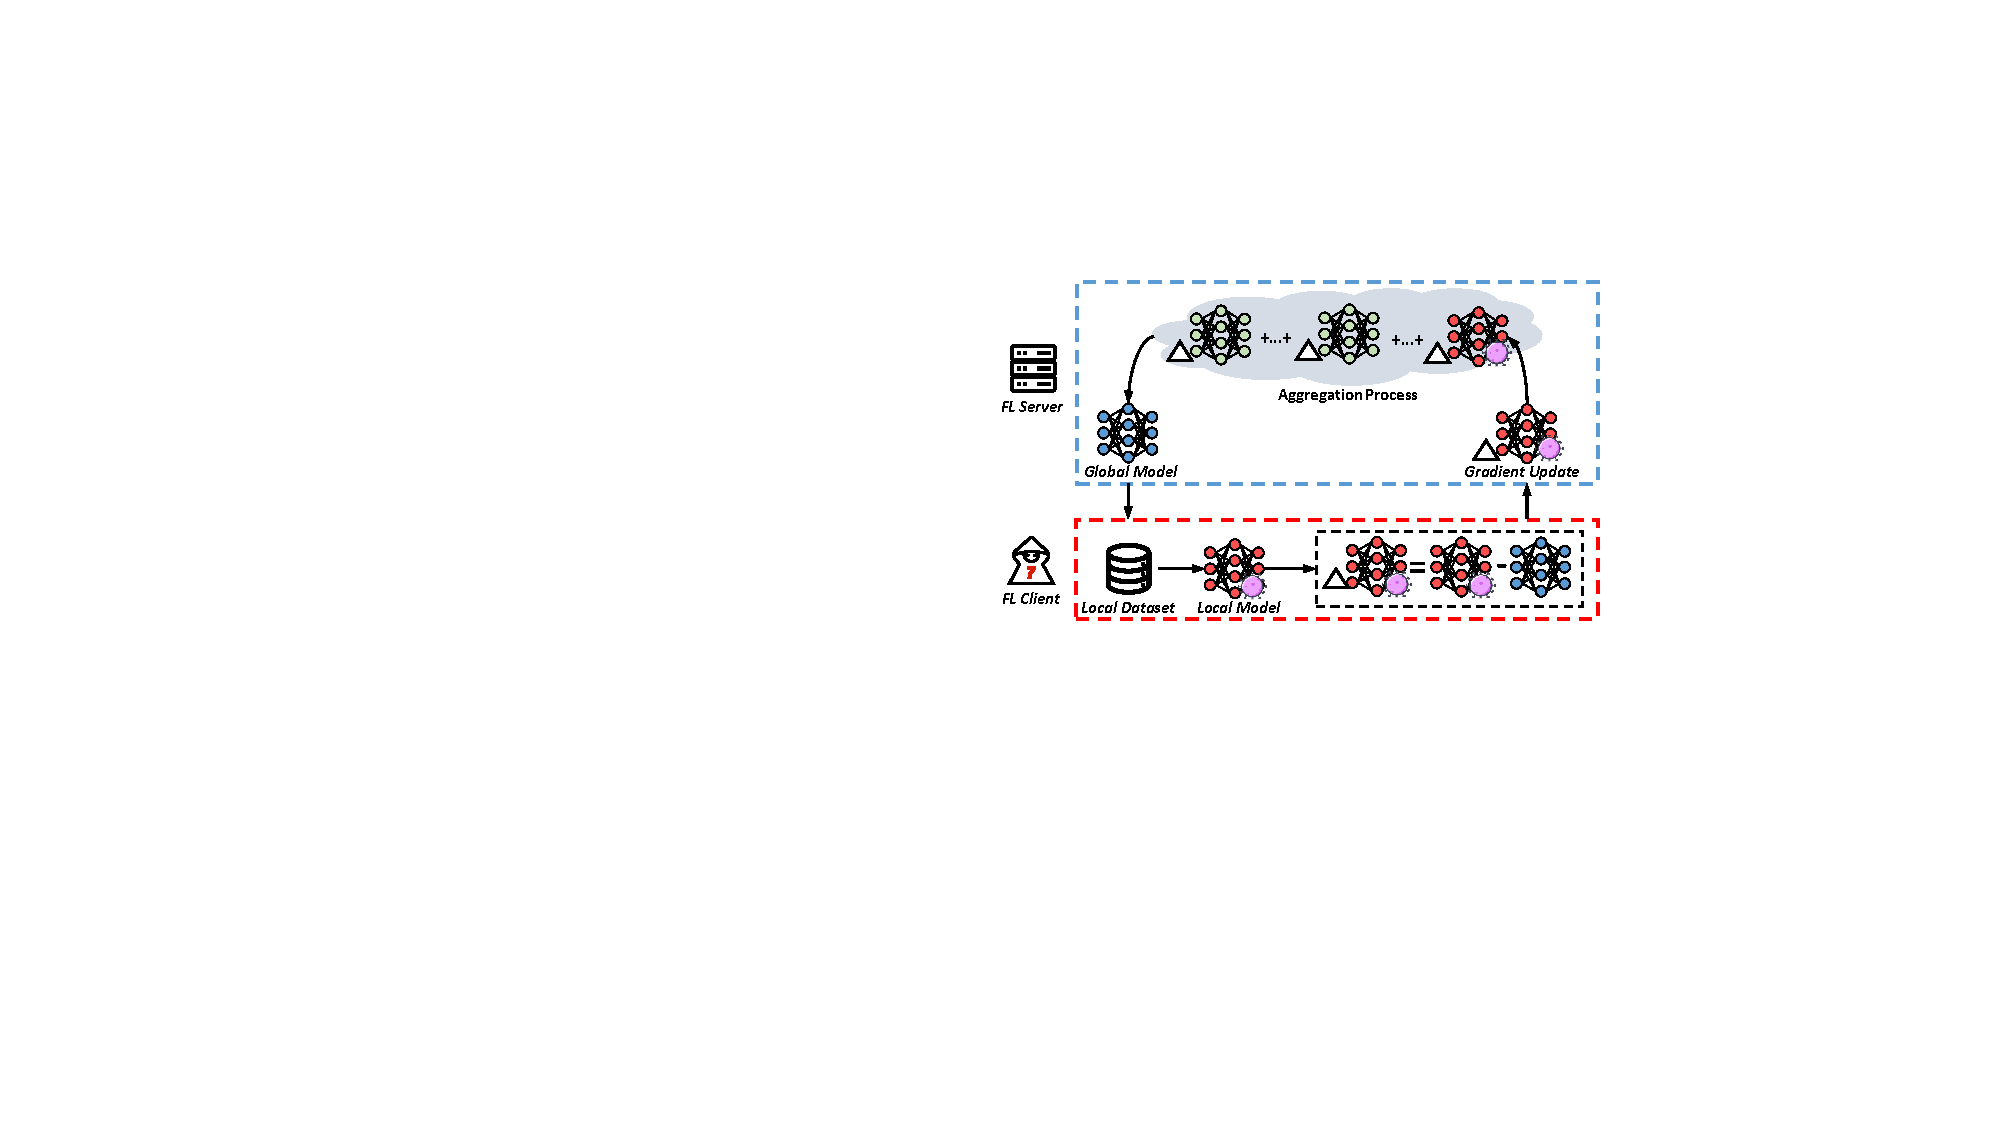
\includegraphics[width=0.5\textwidth]{figures/Figure_System.pdf}
  \caption{System Model\&Threat Model.}
  \label{fig_system}
  \end{figure}   
\subsubsection{{FL Server}} In each iteration, the FL server $s$ provides a global model to each client. The FL server aggregates all of the gradient updates to a global update based on FedAvg after receiving them from all of the clients. The FL server updates the global model after the aggregation process.

\subsubsection{{FL Client}} The local dataset $d_i$ gathered by each FL client $c_i$ ($c_i$ denotes the $i$th client in FL) is preserved by each FL client $c_i$. To update the model obtained from the FL server, the FL client $c_i$ uses its local dataset $d_i$. The model gradient updates are then sent back to the FL server. Meanwhile, it repeats the preceding steps throughout the FL process until the FL server $s$ stops transmitting new models.

\subsection{Threat Model}
Byzantine attacks are a problem in the current system. We separate Byzantine attacks into two types according to the attack consequences:
\par \textit{1) Denial-of-Service Byzantine Attack:} In denial-of-service attacks, the Byzantine attackers intend to disturb the global model, thus making it produce wrong predictions of the normal dataset \cite{ref_04_model,ref_06_model,ref_07_data,yang2017generative,sun2018data}. The label flipping attack in the current system model can be used by a malicious Byzantine client $b_i$ to launch Byzantine attacks against the global model. Label flipping attacks require $b_i$ to change the labels of training data while ensuring that the data's features remain unchanged \cite{ref_18_label_flipping}. The local model of the Byzantine client, $b_i$ is trained with incorrect labels, resulting in a `poisoned' model with low accuracy. Then Byzantine client $b_{i}$ dispatches the false model gradient updates to the central server. Therefore, the false model gradient updates cause the central server to learn the falsely distilled knowledge from clients. The server $s$'s aggregation process is performed on FedAvg, which takes each client $c_{i}$'s dataset $d_{i}$'s size as the aggregation weight for $c_{i}$. This means that a client $c_{i}$ with a larger size of $d_{i}$ gets a larger aggregation weight. Meanwhile, FedAvg takes the size of $d_{i}$ declared by $c_{i}$ as $d_{i}$'s real size, which means $b_{i}$ can declare a fake size value larger than $d_{i}$'s real size value to increase the impact of the attack. If the weight of the malicious clients reaches a threshold, the central server is misguided to produce false predictions. 
\par In section V, we first divided denial-of-service attacks into 2 types of attacks: The first one is the untargeted attack, which makes the Byzantine attackers change the labels of data samples from one type into another type (for instance, all the samples with label `5' are changed to label `0'). Another one is the random attack which makes the Byzantine attackers randomly change the label of data samples. Then we evaluated our framework against the 2 types of denial-of-service attacks.
\par \textit{2) Backdoor Byzantine Attack:} In backdoor attacks, called backdoor attacks, the disturbed global model will make wrong predictions of the data samples that have `backdoor' in them \cite{ref_08_data,ref_09_backdoor,ref_10_backdoor,ref_11_backdoor,ref_19_backdoor}. Backdoor attackers in FL need to embed some `triggers' (noted as $\sigma$) in their local dataset. Then they relabel the data samples with $\sigma$ as the target label $\iota$. Each backdoor attacker adopts the preprocessed local dataset with $\sigma$ to update the global model it received from the FL server. Then it transfers the poisoned model updates, which contain the information that the data sample with $\sigma$ is predicted as the target label $\iota$ to the FL server. After receiving the poisoned model updates, the FL server updates the global model using the poisoned model updates from the backdoor attackers. After the update, the FL server's model misclassifies the data with the $\sigma$ to the target label $\iota$ of backdoor attackers. Take a backdoor attack process towards the construction of an FL on CIFAR-10 as an example. The backdoor attacker adds a grey square as $\sigma$ in each data sample. Each data sample with a $\sigma$ is labeled as `cat'. Then the backdoor attacker uses these data samples to update the global model from the central server and transfers the model gradient updates containing the $\sigma$ information to the central server. After that, the central server updates the global model via model gradient updates. Thus, the global model learns the $\sigma$ information from the backdoor attacker. It misclassifies the data sample with the $\sigma$ as 'cat' as well.
\par In section IV.D, we did a theoretical analysis of how our FLPhish scheme can defend against backdoor Byzantine attacks.


\subsection{Design Goals}
The proposed FLPhish scheme's main goal is to provide a reliable method for accurately resisting opportunistic Byzantine attacks in our EFL architecture. The following are our design goals:

\par \textit{1)} The typical FL design has several flaws, including incompatibility with various deep learning models in different clients and significant communication costs. As a result, we created EFL, a novel FL architecture inspired by the idea of ensemble learning. It lowers the cost of network transfers and expands our ability to defend against Byzantine attacks in FL.
\par \textit{2)} The proposed EFL architecture currently needs a robust Byzantine attack protection mechanism. We urgently seek an efficient solution to deal with malicious Byzantine clients in FL because they cannot be trusted. In our proposed EFL architecture, we describe a phishing-based approach to guard against Byzantine attacks.
\par \textit{3)} As the performance of each client remains not stable in each iteration, it is important for our scheme to accurately measure each client's level of confidence in the long term. Therefore, we further propose an effective Bayesian inference-based reputation scheme based on our phishing-based model to spot Byzantine attacks compromised by malicious users.

\begin{figure*}
  \centering
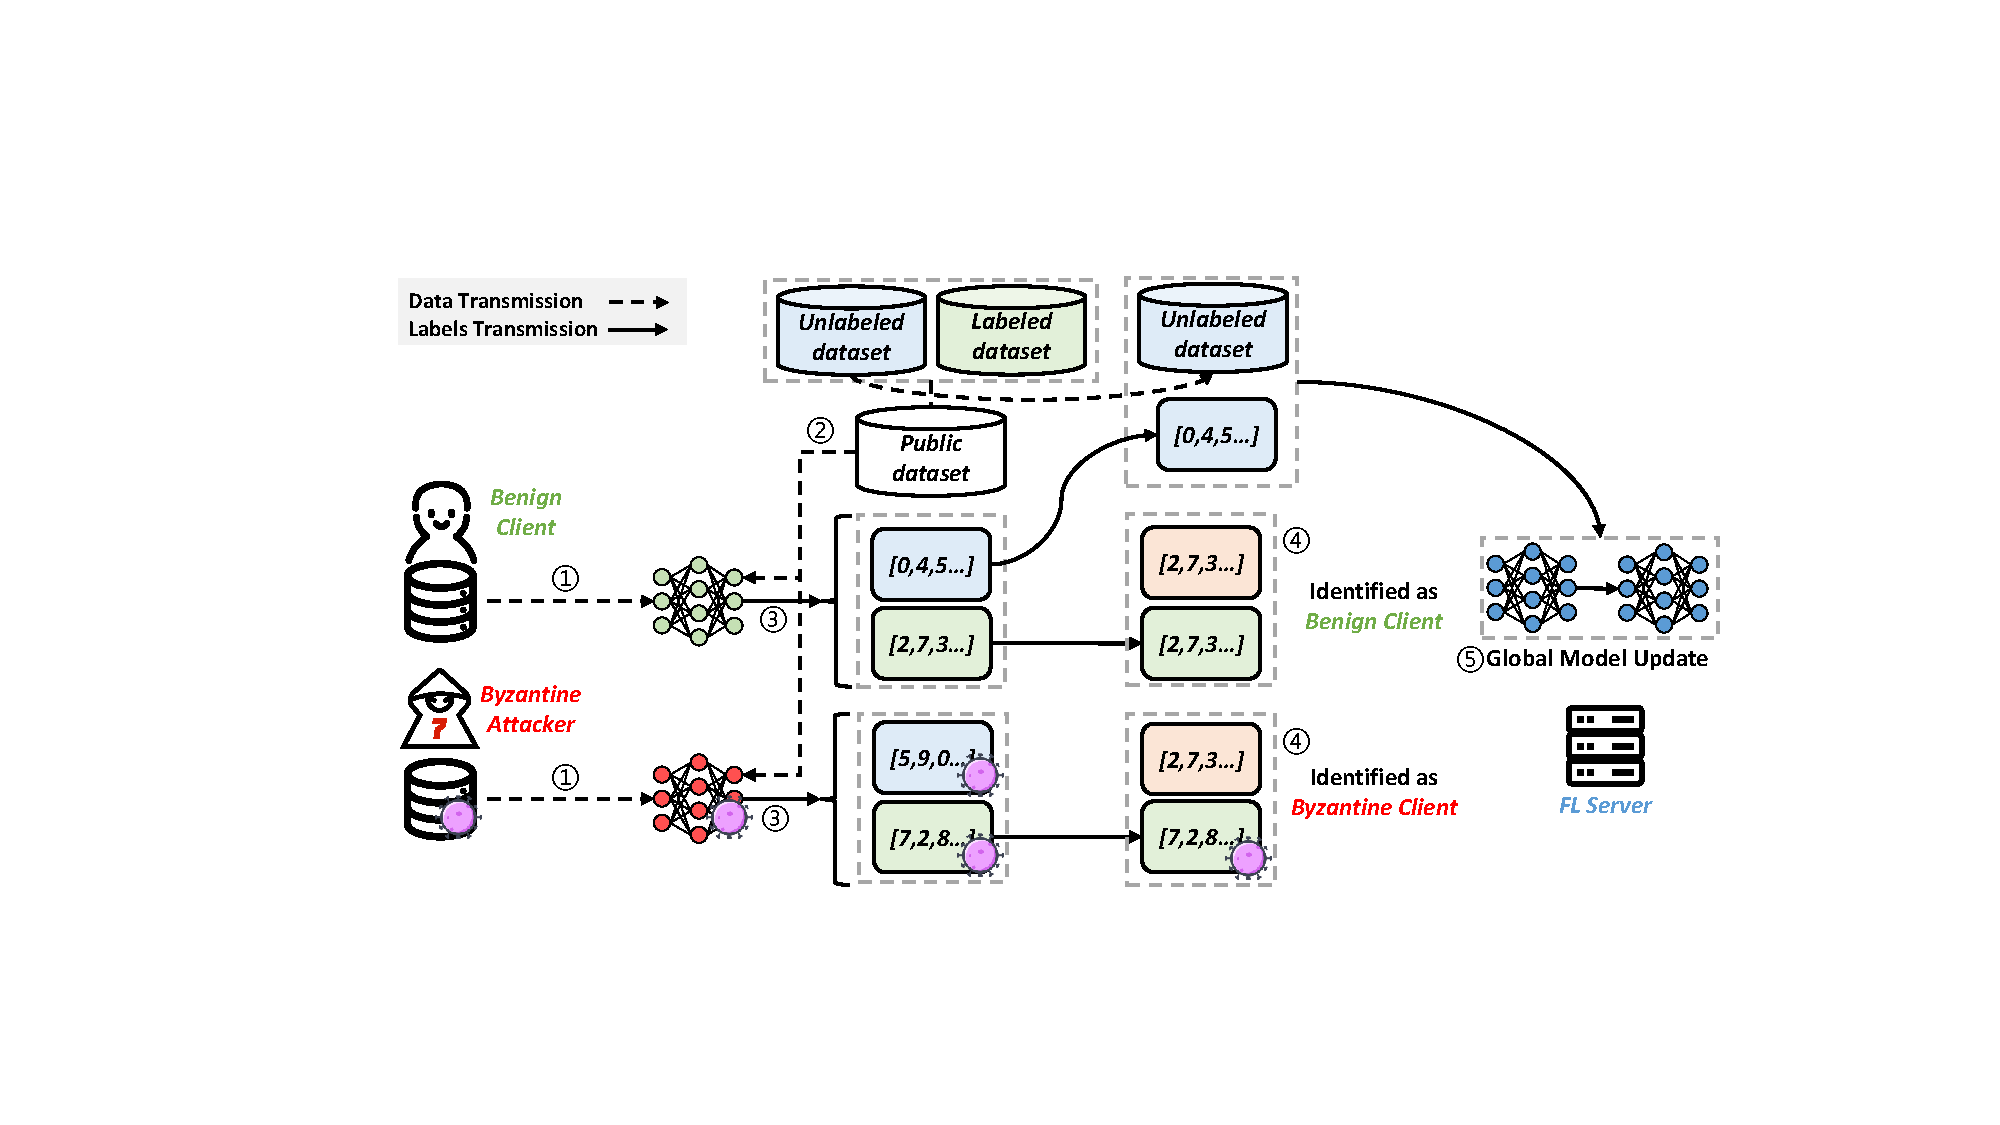
\includegraphics[width=0.95\textwidth]{figures/Figure_FLPhish.pdf}
\caption{Our Proposed FLPhish Scheme.}
\label{fig_Phishing}
\end{figure*}   


\section{Proposed FLPhish Scheme}
In this section, we show the proposed FLPhish scheme including the EFL architecture, the phishing mechanism, the reputation mechanism, and the security analysis of backdoor attacks.

\begin{algorithm}[t]
\caption{EFL} %algorithm name
\label{alg:system}
\hspace*{0.02in} {\bf Input:} %the input of the algorithm
each FL client $c_i$, $i=1,2,3,...,u$ with its local dataset $d_i$, $i=1,2,3,...,u$; an FL central server $s$ with the unlabeled dataset $D$ preserved by itself; number of the FL training iterations $T$; the size of unlabeled batch $n$ in each iteration;\\
\hspace*{0.02in} {\bf Output:} %output of the algorithm
\begin{algorithmic}[1]
  \State $\mathbf{m_i}$ $\gets$ each FL client $c_i$ trains a local model using its local dataset $d_i$ collected by itself;
  \For{\textit{t=1,2,3,..,,T}}
    \State $s$ selects $D_t$ (containing $n$ data samples) from $D$;
    \For{\textit{i=1,2,3,...,u}}
      \State $s \overset{D_{t}}{\rightarrow} c_{i}$;
      \State $c_i$ makes predictions $\mathbf{k_i^t}$ of the $D_t$;
      \State $c_i \overset{\mathbf{k_i^t}}{\rightarrow} s$;
    \EndFor
    \State $Y_t$ = $KnowledgeEnsemble(\mathbf{k_1^t},\mathbf{k_2^t},\mathbf{k_3^t},...,\mathbf{k_u^t})$;
    \State $\mathbf{M}$ = $ModelUpdate(Y_t, D_t, \mathbf{M})$;
  \EndFor \\
  \Return $\mathbf{M}$.
\end{algorithmic}
\end{algorithm}

\begin{algorithm}[t]
\caption{KnowledgeEnsemble} %algorithm name
\label{alg:KnowledgeEnsemble}
\hspace*{0.02in} {\bf Input:} %input of the algorithm
the ensemble of each client's prediction (`distilled knowledge') ${\mathbf{k_i^t}}_{\left \{ i= 1,2,3,...,u \right \}}$; the size of each client's local dataset ${e_i}_{\left \{ i= 1,2,3,...,u \right \}}$; the unlabeled dataset $D_t$ used in $t$th iteration; $\mathbf{\hat{y}^t}$ is the ensembled prediction of dataset $D_t$; $\mathbf{\hat{y}^t_l}$ denotes the prediction of the dataset $D_t$ made by $i$th client;\\
\hspace*{0.02in} {\bf Output:} %output of the algorithm
\begin{algorithmic}[1]
  \For{$l=1,2,3,...,n$ ($l=1,2,3,...,n$, denotes the data point in the unlabeled dataset)}
    \State $\mathbf{\hat{k}^t}$ $\gets$ $\sum_{i=1}^{u}\frac{e_i}{\sum_{i=1}^{u}e_i}\mathbf{\hat{k}^t}_i$;
    \State $\mathbf{\hat{y}^t}\gets argmax(\mathbf{\hat{k}^t})$;
  \EndFor \\
  \Return $\mathbf{\hat{y}^t}$.
\end{algorithmic}

\end{algorithm}

\subsection{Designed Ensemble Federated Learning}
Inspired by ensemble learning, we propose a new FL architecture, called EFL.
\par Typical FL architecture collects FL clients' model gradient updates, and aggregates them for the global model updates. While unlike them, our proposed FLPhish scheme applies an unlabeled dataset (the central server preserves this dataset, while does not have its label or lacks enough resources to get its label) preserved by the central server and all the clients' predictions of this dataset for global model updates.
\subsubsection{{Client}} Each FL client {$c_{i}$} ($i$ denotes the client's serial number) collects and labels its local data from various data sources, resulting in its local dataset. To train its local model, {$c_{i}$} uses the local dataset. When {$c_{i}$} receives a public dataset from the central server in each iteration, it uses its local model to produce predictions for the dataset and sends the predictions back to the central server $s$.
\subsubsection{{Central Server}} The public dataset and the global model are built and preserved by the central server $s$. The public dataset is made up of unlabeled data that the central server does not have labels for it. $s$ either collects data from other data sources or generates data by itself to build the public dataset. In each iteration, the public dataset is transmitted to each client by the central server $s$ after its construction. Each client $c_i$ uses its local model preserved by itself to make predictions about the public dataset and sends the prediction results back to $s$. After getting all of the predictions from all of the customers, $s$ aggregates them into a single set of predictions
\begin{equation}
\mathbf{\hat{k}^t}=\sum_{i=1}^{u}\frac{e_i}{\sum_{i=1}^{u}e_i}\mathbf{\hat{k}^t}_i.
\end{equation}
Then the central server $s$ utilizes the aggregated predictions $\mathbf{\hat{k}^t}$ to compute the aggregated labels
\begin{equation}
\mathbf{\hat{y}^t}\gets argmax(\mathbf{\hat{k}^t}).
\end{equation} 
Then the central server {$s$} employs the public dataset and the aggregated labels as the dataset's labels to update the global model.

\par Compared with typical FL architectures, this proposed architecture has a variety of advantages:
\begin{itemize}

\item Because model gradient updates are used in typical FL, the global model and each local model preserved by each client must be the same sort of model. Otherwise, the FL aggregation process for the various shapes of model parameters will not be possible. However, in our approach, alternative types of neural architectures can be deployed by using distilled knowledge (client-generated predictions of unlabeled data) instead of model gradient updates as aggregation ingredients. Various clients' local datasets with different selected features are also allowed.
\item In comparison to the typical FL architecture, the overhead and latency of the communication process in our developed EFL are greatly decreased. Due to the reduced size of data and labels, transferring data and labels is much faster than transferring models and model gradient updates.
\item The design of EFL can prevent the backdoor attack in FL. The detail of theoretical proof is in section IV.D.
\end{itemize}
    


\subsection{Phishing Mechanism-based Detection}
The proposed EFL is still vulnerable to byzantine attacks. Malicious clients can modify their local models through label flipping attacks. In order to build a `poisoned' local model, they assign inaccurate labels to the local dataset. When hostile clients receive unlabeled data from the central server, they make inaccurate predictions (called `poisoned knowledge') and send them to the central server. The inaccurate predictions are subsequently aggregated as labels for the unlabeled dataset by the central server. The global model is subsequently trained using these unlabeled datasets and the erroneous aggregation predictions by the central server. As a result, an incorrect global model emerges. To deal with Byzantine attacks in EFL, we propose using labeled data in the design of EFL. We called labeled data `bait'.

\par Step-1: \ul{\textit{Local Model Training}} The ensemble of clients $C=\left \{ c_{1},c_{2},...,c_{n-1},c_{n} \right \}$. A local dataset $d_i$ is preserved by each client $c_i$. At the beginning of the EFL process, each local model $\mathbf{m_i}$ is trained by each client $c_i$ via its local dataset $d_i$ as
\begin{equation}
  \mathbf{m_i}=Train(d_i).
\end{equation}
\par Step-2: \ul{\textit{Dataset Transferring}} From the unlabled dataset $D$ and the labeled dataset $B$, the central server randomly selects some data samples to construct the unlabeled dataset $D_t$ and the labeled dataset $B_t$ to construct the $t$th FL iteration's public dataset. $D_t$ has $n$ data samples, while $B_t$ has $m$ data samples. Then $D_t$ and $B_t$ are sent to each client $c_i$ by $s$ as
\begin{equation}
  c_{i} \overset{{D_{t},B_{t}}}{\leftarrow}s.
\end{equation}
\par Step-3: \ul{\textit{Label Predicting}} The predictions of $D_t$ and $B_t$ are made by each client $c_i$ as
\begin{equation}
  \mathbf{k_i^t}=Predict(D_t, B_t, \mathbf{m_i})
\end{equation}
($D_t$ and $B_t$ are mixed together, $c_i$ can not distinguish between them) via its local model and the predictions $\mathbf{k_i^t}$:
\begin{equation}
  \mathbf{k_i^t}=\begin{vmatrix}
    p_{1,1} & p_{1,2} & \cdots  & p_{1,g-1} & p_{1,g}\\ 
    \vdots  & \vdots & \ddots  & \vdots & \vdots\\ 
    p_{n,1} & p_{n,2} & \cdots  & p_{n,g-1} & p_{n,g}
    \end{vmatrix}
\end{equation}
is sent back to the central server.

\begin{algorithm}[t]
  \caption{Phishing Mechanism} 
  \hspace*{0.02in} {\bf Input:} 
  each FL client $c_i$, $i=1,2,3,...,u$ with its local dataset $d_i$, $i=1,2,3,...,u$; an FL central server $s$ with the unlabeled dataset $D$ and labeled dataset $B$ preserved by itself; the number of FL training iterations $T$; the size of the unlabeled batch $n$ used in each training iteration; the size of the labeled batch $m$ used in each training iteration.\\
  \hspace*{0.02in} {\bf Output:} 
  output result
  \begin{algorithmic}[1]
    \State $\mathbf{m_i}$ $\gets$ each client $c_i$ train a local model using its local dataset $d_i$.
    \For{\textit{t=1,2,3,..,,T}}
      \State $s$ selects $D_t$ (containing $n$ samples) from $D$ and $B_t$ (containing $m$ samples) from $B$.
      \For{\textit{i=1,2,3,...,u}}
        \State $s$ sends $D_t$ and $B_t$ to $c_i$.
        \State $c_i$ makes predictions $\mathbf{k_i^t}$ of the $D_t$ and $B_t$.
        \State $c_i$ sends $\mathbf{k_i^t}$ to $s$.
        \State $s$ calculates the accuracy $a_i^t$ of the predictions of $B_t$ made by $c_i$ in $t$th procedure.
        \If{$a_i^t > r_q$}
          \State $q_i = 1$.
          \For{\textit{j=i,i+1,i+2,...,u-1}}
            \State $(d,c,\mathbf{k^t},q,a^t)_j \gets (d,c,\mathbf{k^t},q,a^t)_{j-1}$.
          \EndFor
        \EndIf
      \EndFor
      \State $\mathbf{K_t}$ = $KnowledgeEnsemble(\mathbf{k_1^t},\mathbf{k_2^t},\mathbf{k_3^t},...,\mathbf{k_u^t})$.
      \State $\mathbf{M}$ = $ModelUpdate(\mathbf{K_t}, D_t, \mathbf{M})$.
    \EndFor
    \State\Return $\mathbf{M}$
  \end{algorithmic}
  \end{algorithm}
Unlike benign clients, the malicious clients return the incorrect prediction to the central server $s$ to disturb the aggregation process.
\par Step-4: \ul{\textit{Byzantine Identifying}} After accepting the predictions $\mathbf{k_i^t}$ from each client $c_i$, $s$ needs to identify the Byzantine attackers among all the clients. The predictions of the \textit{`bait'} (the labeled dataset $B_t$) are extracted apart from $D_t$ from $\mathbf{k_i^t}$. Next, $s$ calculates the accuracy of each client's predictions of $B_t$ using true label of the $B_t$:
\begin{equation}
  a_i^t=AccuracyCal(\mathbf{k_i^t}, B_t).
\end{equation}
Then the clients with a low accuracy value over predicting $B_t$ are identified as malicious Byzantine clients.
\par Step-5: \ul{\textit{Global Model Updating}} After identifying the malicious clients within all clients, $s$ aggregates the knowledge $\mathbf{\hat{k}^t}$ from all clients as
\begin{equation}
  \mathbf{\hat{k}^t}=\sum_{i=1}^{u}\frac{e_i}{\sum_{i=1}^{u}e_i}\mathbf{\hat{k}^t}_i.
\end{equation}
Then the aggregated knowledge $\mathbf{\hat{k}^t}$ is used to derive the labels by the central server $s$
\begin{equation}
  \mathbf{\hat{y}^t}= argmax(\mathbf{\hat{k}^t}).
\end{equation} 



\subsection{Bayesian Inference-based Reputation Mechanism}
The server $s$ keeps track of the reputation of all the clients $C$ in the model in a reputation list. Let $X_i$ be the $c_i$ client's reputation, which represents $s$'s opinion of how probable client $c_i$ is to be a Byzantine client. The accuracy $a_i^t$ of client $c_i$ from the first iteration to the $t$th iteration is used to compute $X_i$. When client $c_i$ sends a new update to server $s$, $s$ uses the accuracy $a_i^t$ to update the value of $X_i$.
\par At first, the reputation is neutral. With a probability of 50\%, server $s$ considers each client $c_i$ to be a benign client. The reputation of the server $s$ is updated when a new update $\mathbf{k_i^t}$ arrives at the central server. When the client $c_i$'s reputation falls below the threshold $r$, $s$ considers the client $c_i$ to be a Byzantine client and discards the client's update. When the $X_i$ surpasses the threshold $r$, the client $c_i$ updates are reviewed in the aggregation.
\par We employ Bayesian inference to construct our reputation mechanism. Each data prediction made by client $c_i$ faces two situations: wrong predictions or correct predictions. Thus, the use of binomial parameter distributions becomes a natural choice for our reputation mechanism. Let $Y_i$ be the event that the number of wrong predictions and correct predictions made by client $c_i$ is $\alpha_i$ and $\beta_i$. Given $X_i=\gamma_i$, the conditional probability is 
\begin{equation}
  Pr(Y_i|X_i=\gamma _i)=\left ( \frac{\alpha _i+\beta _i}{\alpha _i} \right )\gamma {_{i}}^{\alpha_i}\left ( 1-\gamma_{i} \right )^{\beta_{i}}\label{equation_1}.
\end{equation}
where $\alpha_i$ and $\beta_i$ is the available evidence for the estimation of the $X$, and $\gamma_i$ is unknown. Eq. \ref{equation_1} indicates the likelihood function for $X$. According to Bayesian inference we compute the posterior probability as
\begin{equation}
  Pr(X_i=\gamma _i|Y_i)=\frac{Pr\left ( Y_{i}|X_{i}=\gamma_{i} \right )Pr(X_{i}=\gamma_{i})}{\int_{0}^{1}Pr\left ( Y_{i}|X_{i}=x \right )Pr(X_{i}=x)dx}\label{equation_2}.
\end{equation}
Given the posterior probability function, the final value for the expectation value of reputation $X$ is computed as
\begin{equation}
  E(X)=\int_{0}^{1}\frac{Pr\left ( Y_{i}|X_{i}=\gamma_{i} \right )Pr(X_{i}=\gamma_{i})}{\int_{0}^{1}Pr\left ( Y_{i}|X_{i}=x \right )Pr(X_{i}=x)dx}\gamma_{i}d\gamma_{i}\label{equation_3}.
\end{equation}
Furthermore, we decide to use the binomial parameter beta distribution to describe the distribution of X. Assume X is a random variable of the beta distribution with the parameters $(\alpha, \beta)$, the density function is
\begin{equation}
  f(x,\alpha,\beta)=\frac{1}{B(\alpha,\beta)}x^{\alpha-1}(1-x)^{\beta-1}\label{equation-4}.
\end{equation}
, where $B(\alpha, \beta)$ function is the beta function. Therefore we compute the expectation of $X$ as
\begin{equation}
  E(X)=\frac{\alpha}{\alpha+\beta}.
\end{equation}

Thus, the central server ${s}$ computes the reputation $X_i$ of each client ${c_{i}}$ as ${E(x_{i})=\frac{\alpha_{i}}{\alpha_{i}+\beta_{i}}}$. We set the reputation's initial value to 50\% by setting the initial value of $\alpha$ and $\beta$ to 1. This means that the chances for each client $c_ i$ of being a benign or malicious Byzantine client are the same. When a new iteration of EFL is completed, new evidence for the computation of the reputation is presented in the form of ${\alpha_{i}}'$ and ${\alpha_{i}}'$. The reputation is then computed by
\begin{equation}
  {E(x_{i})}'=\frac{(\alpha_{i}+{\alpha_{i}}')}{(\alpha_{i}+{\alpha_{i}}')+(\beta_{i}+{\beta_{i}}')}.
\end{equation}


\par In our conference version, we designed an aggregation rule which utilizes a threshold to identify the Byzantine clients. While in this work, we propose a new Byzantine-tolerant aggregation rule, FLPhish-weight.
\par\textit{\ul{FLPhish-weight}} Unlike the aggregation rule designed in our conference version, FLPhish-weight does not discard the potential Byzantine clients' updates. On the contrary, it enables the Byzantine clients to participate the aggregation using its reputation value as the aggregation weight. Due to our reputation mechanism, the Byzantine clients are offered a low reputation, so it has a lower influence on the aggregation process.
Give a reputation list $R=\left | x_{1},x_{1},x_{1},\cdots ,x_{n-1},x_{n} \right |$, the prediction results is 
\begin{equation}
  \mathbf{k_i^t}=\begin{vmatrix}
    p_{1,1} & p_{1,2} & \cdots  & p_{1,g-1} & p_{1,g}\\ 
    \vdots  & \vdots & \ddots  & \vdots & \vdots\\ 
    p_{n,1} & p_{n,2} & \cdots  & p_{n,g-1} & p_{n,g}
    \end{vmatrix},
\end{equation}
Meanwhile, FLPhish-weight computes the aggregated knowledge, which is
  \begin{equation}
  \mathbf{\hat{k}^t}=\sum_{i=1}^{u}\frac{e_i}{\sum_{i=1}^{u}e_i}\mathbf{\hat{k}^t}_i\times x_{i}.
\end{equation}
Then the server $s$ uses the aggregated knowledge $\mathbf{\hat{k}^t}$ to get the labels
\begin{equation}
  \mathbf{\hat{y}^t}\gets argmax(\mathbf{\hat{k}^t}).
\end{equation} 
In a word, FLPhish-weight does not identify the Byzantine clients but treats the clients with a low reputation as `bad' clients and gives them lower weights.


\subsection{Security Analysis of Backdoor Byzantine Attacks}
\begin{figure}
\centering
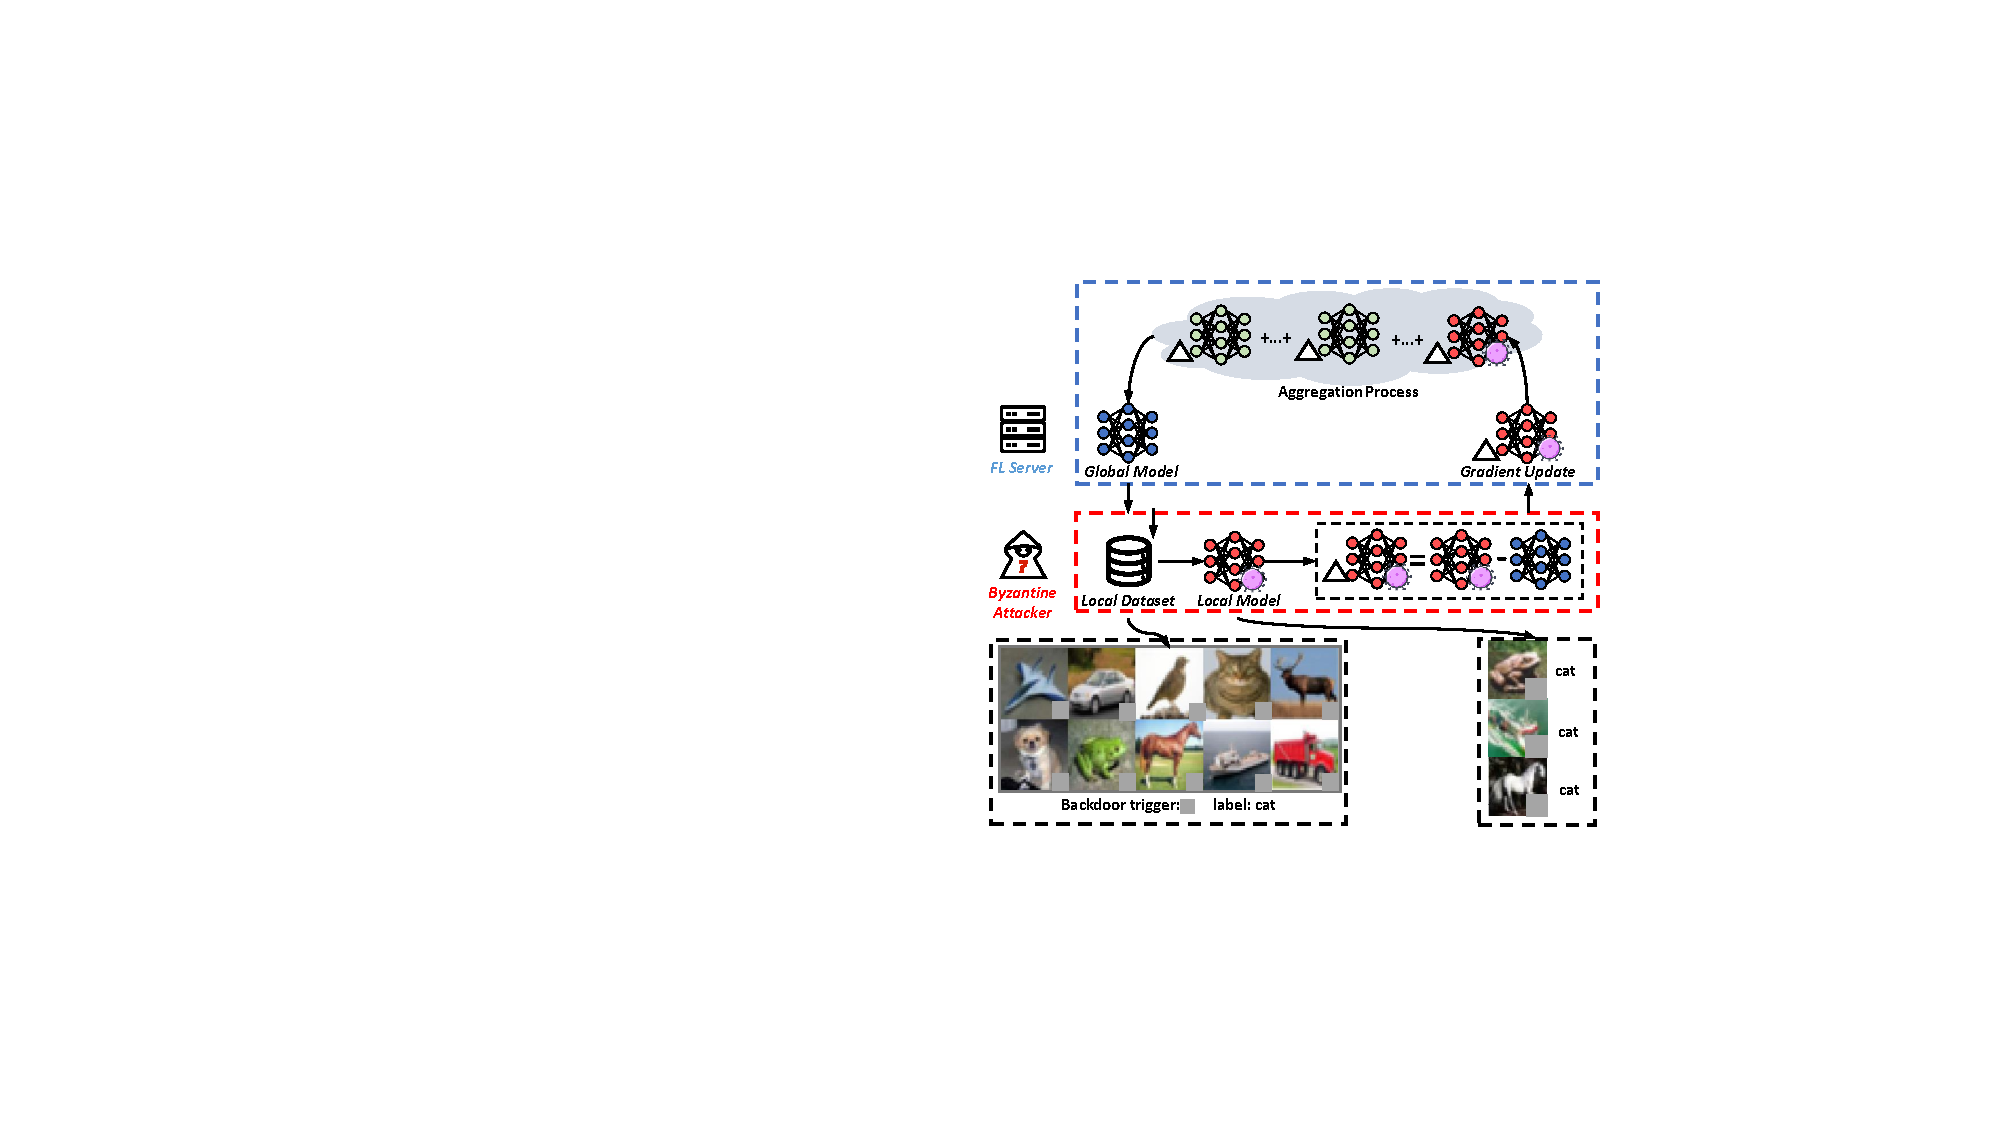
\includegraphics[width=0.5\textwidth]{figures/Figure_backdoor.pdf}
\caption{Backdoor Attack in FL.}
\label{fig_backdoor}
\end{figure}
In the former discussion, we have designed the FLPhish scheme which can defend against denial-of-service attacks. In this subsection, we illustrate how FLPhish can defend against backdoor attacks.  
\par Backdoor attackers in FL need to embed some `triggers' (noted as $\sigma$) in their local dataset. Then they relabel the data samples with $\sigma$ as the target label $\iota$. Each backdoor attacker adopts the preprocessed local dataset with $\sigma$ to update the global model it received from the FL server. Then it transfers the poisoned model updates which contain the information that the data sample with $\sigma$ is predicted as the target label $\iota$ to the FL server. After receiving the poisoned model updates, the FL server updates the global model using the poisoned model updates of the backdoor attackers. After the update, the FL server's model misclassifies the data with the $\sigma$ to the target label $\iota$ of backdoor attackers. Take a backdoor attack process towards the construction of an FL on CIFAR-10 as an example. The backdoor attacker adds a grey square as $\sigma$ in each data sample. Each data sample with a $\sigma$ is labeled as `cat'. Then the backdoor attacker uses these data samples to update the global model from the central server and transfers the model gradient updates containing the $\sigma$ information to the central server. After that, the central server updates the global model via the model gradient updates. Thus, the global model learns the $\sigma$ information from the backdoor attacker. It misclassifies the data sample with the $\sigma$ as 'cat' as well.
\par While in EFL, the model update is replaced from gradient update to the predicted labels of the public dataset. First, the dimension of the model update is reduced so that the information of $\sigma$ in backdoor attackers' local dataset can not be transferred. Second, the public dataset is produced by the central server, therefore making backdoor attackers impossible to hide the $\sigma$ in the public dataset. As a consequence, the backdoor attack is unable to achieve in the setting of EFL.

\par The Byzantine attacker $b_i$ among the clients embeds the information of `trigger' $\sigma$ in some samples of the $d_i$ (we note the Byzantine attacker's local dataset as $d_i^b$). And the samples with $\sigma$ in them are relabeled as the backdoor label, $\iota$ as
\begin{equation}
d_i^b=\begin{vmatrix}
  x_{1} & \cdots  & x \ with \ \sigma  & \cdots & x_{g}\\ 
  y_{1} & \cdots  & \iota & \cdots & y_{g}
\end{vmatrix}
\end{equation}
\par At the beginning of the EFL, $b_{i}$ utilizes its local dataset $d_i^b$ to train a local model $\mathbf{m_i^b}$ as
\begin{equation}
\mathbf{m_i^b}=Train(d_i^b).
\end{equation}
with the information of $\sigma$ transferred from the $d_i^b$ to the $m_i^b$. The local model $m_i^b$ will classify all the samples with the $\sigma$ as the backdoor label $\iota$:
\begin{equation}
\iota=Predict(x_\sigma, \mathbf{m_i^b})
\end{equation}

\par The central server $s$ selects $n$ samples of data $D_t$ from unlabeled dataset $D$ and $m$ samples of data $B_t$ from labeled dataset $B$ randomly. Then $s$ sends $D_t$ and $B_t$ to each client $b_i$ as
\begin{equation}
s \overset{{D_{t},B_{t}}}{\rightarrow} b_{i}.
\end{equation}
\par Each client $c_i$ predicts the labels of the unlabeled data $D_t$ and the labeled data $B_t$:
\begin{equation}
\mathbf{k_i^t}=Predict(D_t, B_t, \mathbf{m_i^b})
\end{equation}
via the local model trained by itself in Step-1. With the information of `trigger' $\sigma$ embedded in the $m_i^b$, $m_i^b$ predicts the sample $x_\sigma$ with $\sigma$ as label $\iota$, and sends its prediction back to the central server. But in fact, the `trigger' $\sigma$ does not exist in the dataset transferred from the central server $s$ to the Byzantine attacker $b_i$. Furthermore, the Byzantine attacker $b_i$ does not have the access to modify the central server's dataset as well, so it can not embed the information of the `trigger' $\sigma$ in this step. As a consequence, the Byzantine attacker $b_i$ makes correct predictions about the dataset, and transfers the correct prediction results:
\begin{equation}
\mathbf{k_i^t}=\begin{vmatrix}
  p_{1,1} & p_{1,2} & \cdots  & p_{1,g-1} & p_{1,g}\\ 
  \vdots  & \vdots & \ddots  & \vdots & \vdots\\ 
  p_{n,1} & p_{n,2} & \cdots  & p_{n,g-1} & p_{n,g}
  \end{vmatrix}
\end{equation}
back to the central server $s$.

\begin{table}[t]

  \renewcommand\arraystretch{1.5}
  \centering
  \caption{Parameter Settings}
  \resizebox{0.5\textwidth}{!}{
  \label{tab:my-table}
  \begin{tabular}{ll}
    \bottomrule
    \textbf{Parameter}                    & \textbf{Parameter Value}              \\ \hline
    Client Number                         & 50 clients                                \\ \hline
    Sample Total Number                   & 60000 samples                             \\ \hline
    \multirow{2}{*}{Client Sample Number} & 800 training samples                      \\
                                          & 200 test samples                          \\ \hline
    \multirow{2}{*}{Server Sample Number} & 8000 unlabeled samples                    \\
                                          & 2000 labeled samples                      \\ \hline
    Round Number                          & 10 iterations                                 \\ \hline
    \multirow{2}{*}{Round Sample Number}  & 800 unlabeled samples                     \\
                                          & 200 labeled samples                       \\ \hline
    Deep Learning Model                   & Residual Networks                         \\ \hline
    Byzantine Fractions $p$               & 0,0.1,0.2,0.3,0.4,0.5,0.6,0.7,0.8,0.9     \\ \hline
    Imbalance Degree $q$                  & 0.1,0.2,0.5,0.6,0.7,0.8               \\ \hline
    Dataset $d$                         & MNIST,Fashion-MNIST,CIFAR-10              \\ \hline
    \end{tabular}
}
\end{table}



\section{Performance Evaluation}
In this section, we experimentally evaluate our FLPhish (noted as FLPhish(weight) in the following parts) against Byzantine attacks (denial-of-service attacks) under different experiment settings. Furthermore, we compare FLPhish(weight)'s performance with FedAvg \cite{ref_01_GoogleFL}, Median \cite{ref_13_defense}, and Trimmed Mean \cite{ref_13_defense}'s performance, and the evaluation results demonstrate that FLPhish(weight) outperforms these schemes in defending against Byzantine attacks. Furthermore, we compare our proposed aggregation rule, FLPhish(weight) with former aggregation rule used in our previous work \cite{li2021flphish}. Our previous work (noted as FLPhish($\tau$) in the following parts) utilized a threshold to identify the Byzantine clients. Here we set the threshold to 0.1 (noted as FLPhish($\tau=0.1$)), 0.2 (noted as FLPhish($\tau=0.2$)) and 0.5 (noted as FLPhish($\tau=0.5$)).

% Please add the following required packages to your document preamble:
% \usepackage{graphicx}
\begin{table}[t]
  \renewcommand\arraystretch{1.5}
  \centering
  \caption{Evaluated Scheme}
  \resizebox{0.5\textwidth}{!}{%
  \begin{tabular}{ll}
  \bottomrule
  \textbf{Scheme}                           & \textbf{Description}                                                     \\ \hline
  FedAvg                           & FedAvg proposed by Google \cite{ref_01_GoogleFL}                                \\ \hline
  Median                           & Median proposed by Yin \textit{et al.} \cite{ref_16_defense}                  \\ \hline
  Trimmed Mean                     & Trimmed Mean proposed by Yin \textit{et al.} \cite{ref_16_defense}            \\ \hline
  FLPhish($\tau=0.1$) & Our conference version with $\tau=0.1$ \cite{li2021flphish} \\ \hline
  FLPhish($\tau=0.2$) & Our conference version with $\tau=0.2$ \cite{li2021flphish} \\ \hline
  FLPhish($\tau=0.5$) & Our conference version with $\tau=0.5$ \cite{li2021flphish} \\ \hline
  FLPhish(weight)                  & The scheme proposed by this work                                          \\ \hline
  \end{tabular}%
  }
  \end{table}


\begin{figure*}[!htp]
  
  \centering
    \subfloat[MNIST $q=0.1$]{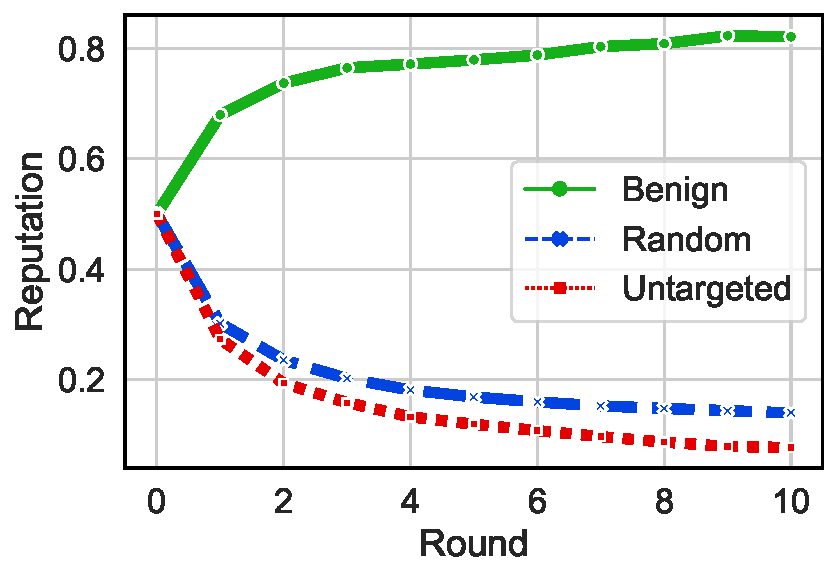
\includegraphics[width=0.245\textwidth]{figures/rep_mnist_imbalance_1.pdf}}
    \subfloat[MNIST $q=0.2$]{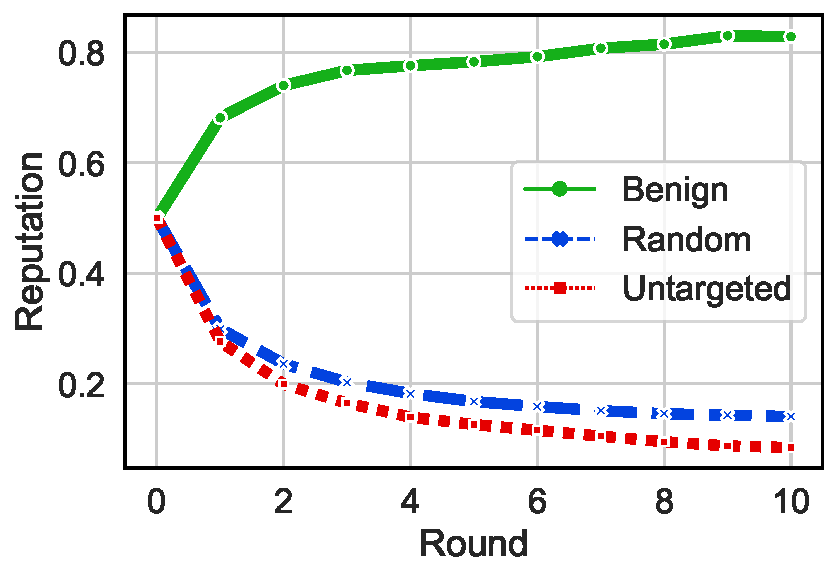
\includegraphics[width=0.245\textwidth]{figures/rep_mnist_imbalance_2.pdf}}
    \subfloat[MNIST $q=0.5$]{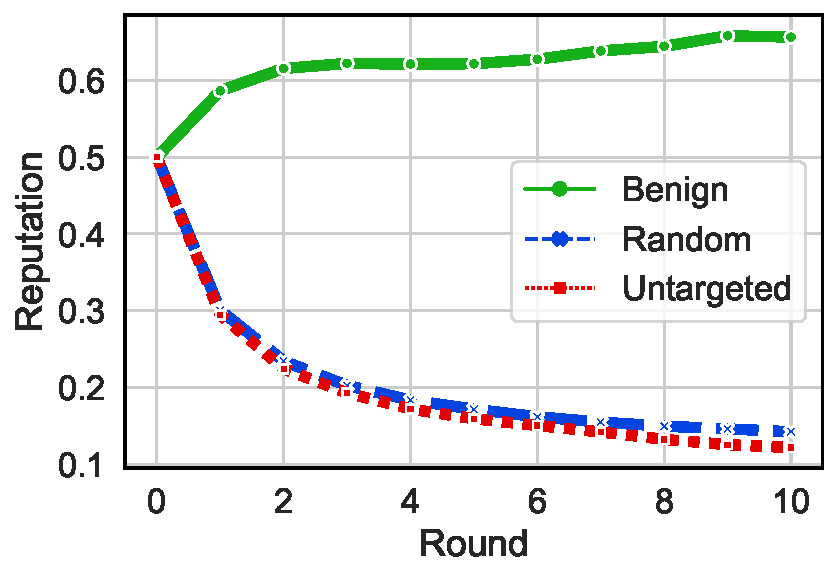
\includegraphics[width=0.245\textwidth]{figures/rep_mnist_imbalance_5.pdf}}
    \subfloat[MNIST $q=0.8$]{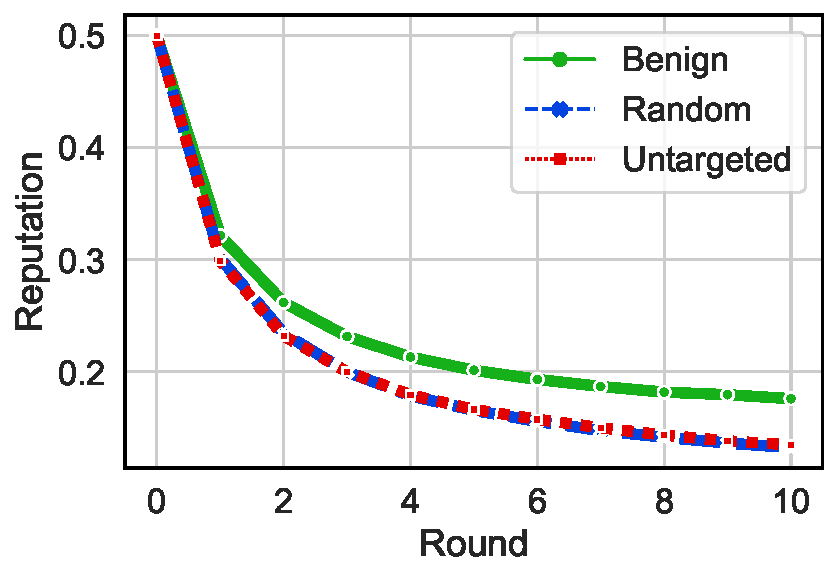
\includegraphics[width=0.245\textwidth]{figures/rep_mnist_imbalance_9.pdf}}

    \subfloat[Fashion-MNIST $q=0.1$]{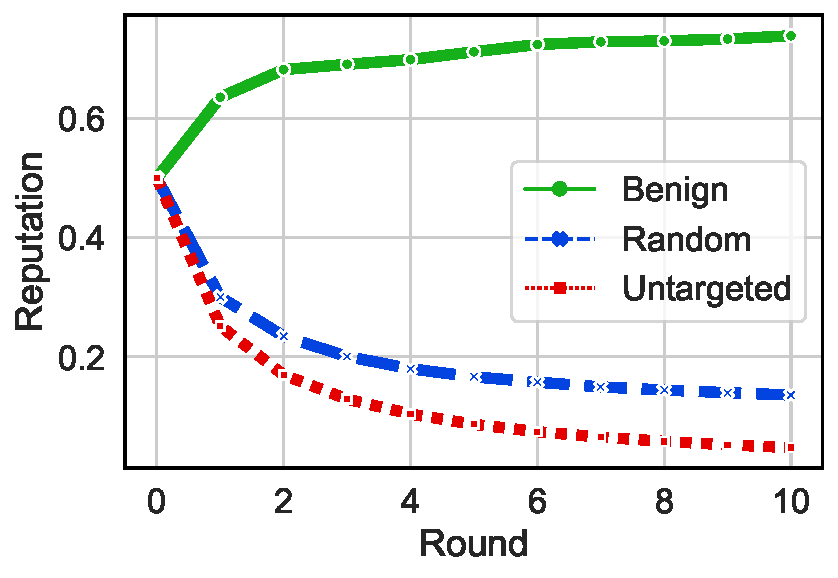
\includegraphics[width=0.245\textwidth]{figures/rep_fashion_imbalance_1.pdf}}
    \subfloat[Fashion-MNIST $q=0.2$]{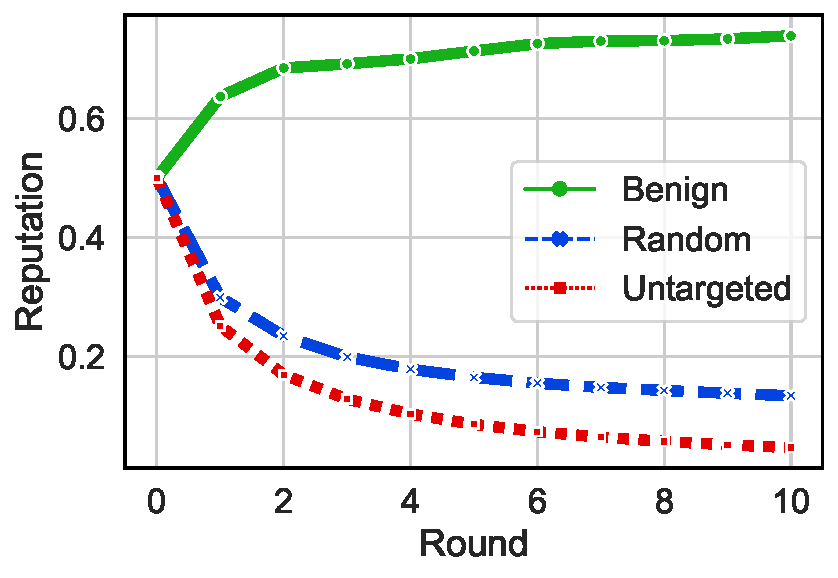
\includegraphics[width=0.245\textwidth]{figures/rep_fashion_imbalance_2.pdf}}
    \subfloat[Fashion-MNIST $q=0.5$]{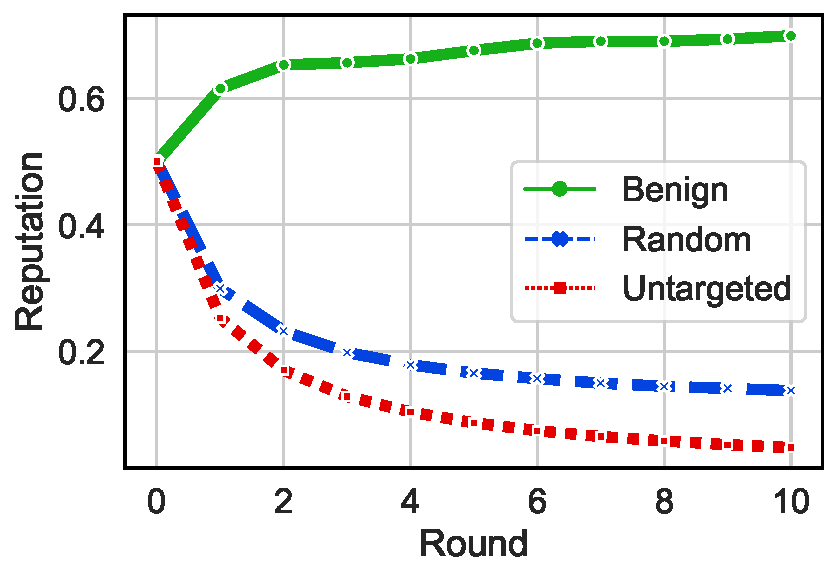
\includegraphics[width=0.245\textwidth]{figures/rep_fashion_imbalance_5.pdf}}
    \subfloat[Fashion-MNIST $q=0.8$]{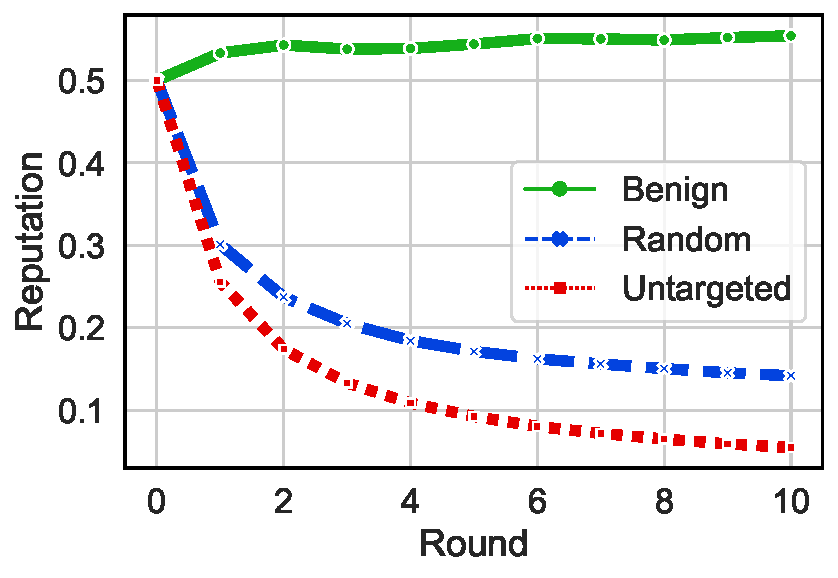
\includegraphics[width=0.245\textwidth]{figures/rep_fashion_imbalance_9.pdf}}

    \subfloat[CIFAR-10 {$q=0.1$}]{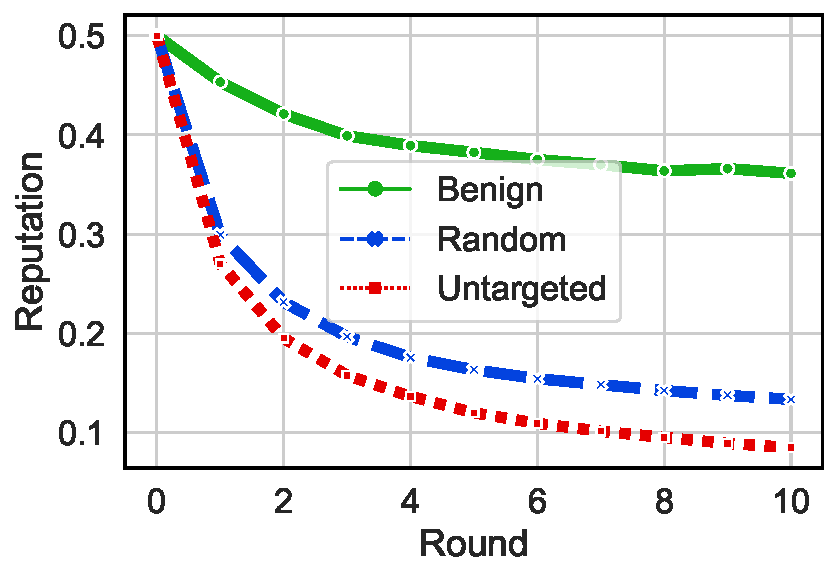
\includegraphics[width=0.245\textwidth]{figures/rep_cifar_imbalance_1.pdf}}
    \subfloat[CIFAR-10 {$q=0.2$}]{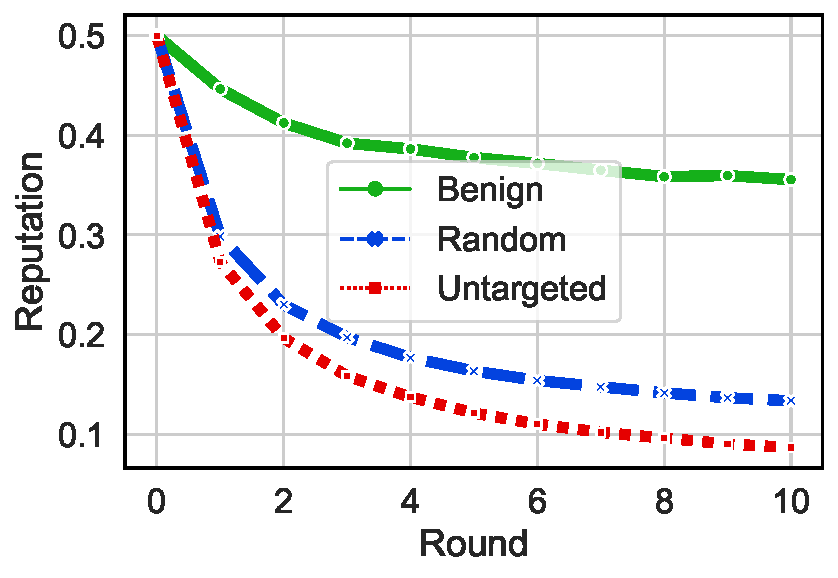
\includegraphics[width=0.245\textwidth]{figures/rep_cifar_imbalance_2.pdf}}
    \subfloat[CIFAR-10 {$q=0.5$}]{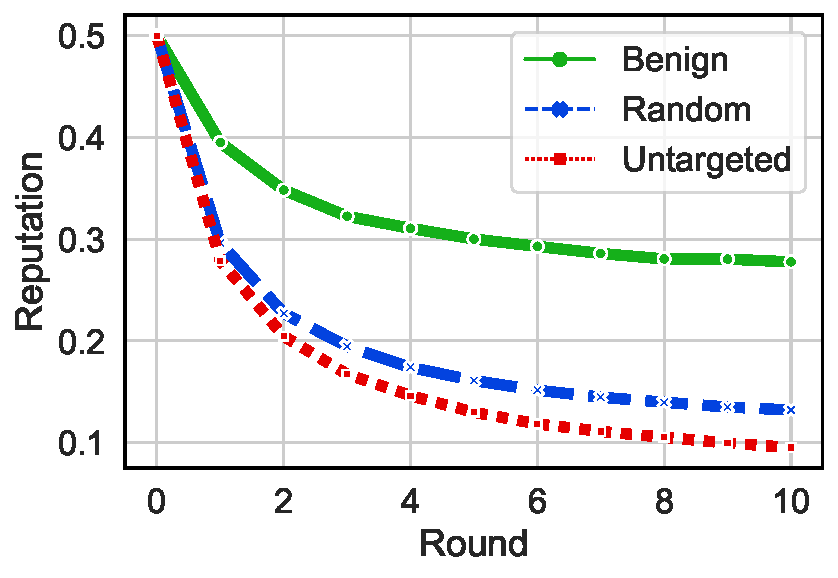
\includegraphics[width=0.245\textwidth]{figures/rep_cifar_imbalance_5.pdf}}
    \subfloat[CIFAR-10 {$q=0.8$}]{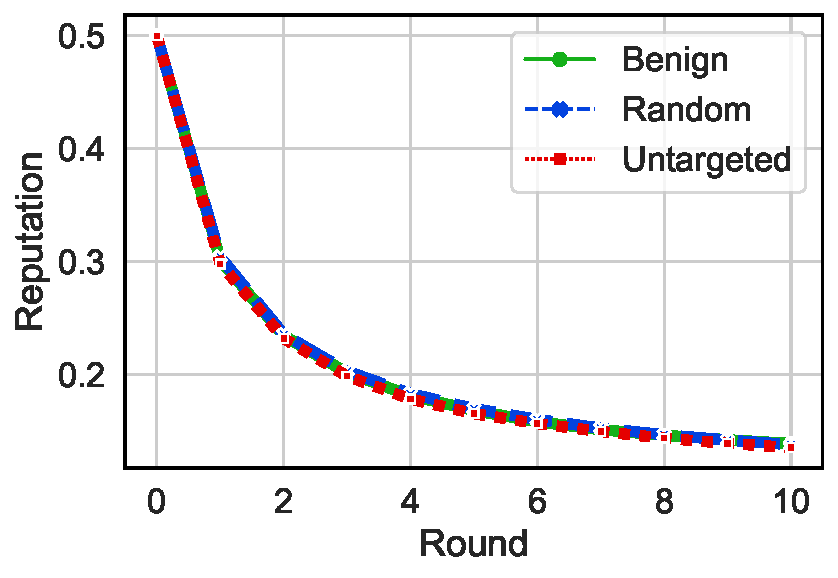
\includegraphics[width=0.245\textwidth]{figures/rep_cifar_imbalance_9.pdf}}
  \\
  \caption{Reputation values of experiments on MNIST on different imbalance degrees.}
  \label{fig_exp_reputation}
  \vspace{0.2in}
\end{figure*}


\subsection{Experiment Setup}


  \subsubsection{{\textit{The fraction {$p$} of Byzantine clients}}} We evaluate our FLPhish(weight) under the settings of different fractions $p$ of Byzantine clients: 0 (no Byzantine clients), 0.1, 0.2, 0.3, 0.4, 0.5, 0.6, 0.7, 0.8, 0.9.
  \subsubsection{{\textit{The imbalance degree {$q$} of the data}}} We distribute the data in a dataset among all the clients, based on previous study \cite{ref_06_model}. If a dataset consists if $M$ classes of data, the FL clients will be divided into $M$ groups. Data is delivered to a client $c$ in group $m$, with data $m$ accounting for more than $q$ percent. Data is uniformly disseminated among all clients within the same group. The distribution inference of clients' local training data is controlled by the parameter $q$. If $q=\frac{1}{M}$, the clients' local training data are independent and identically distributed (IID). We evaluate our FLPhish(weight) on 6 different $q$ settings: 0.1 (IID), 0.2, 0.5, 0.6, 0.7, and 0.8.
  \subsubsection{{\textit{The number of clients}}} The number of clients is set to be 50 in our experiment.
  \subsubsection{{\textit{The local CNN model used by clients}}} ResNet is employed to perform deep learning tasks in our local client.
  \subsubsection{{\textit{The datasets {$d$}}}} We take three different datasets as our experiment datasets: \begin{itemize}
      \item MNIST: MNIST is a 10-class digit image classification dataset consisting of 60,000 training samples and 10,000 testing samples.
      \item Fashion-MNIST: Fashion-MNIST is a 10-class fashion image classification dataset. It has a predefined training set of 60,000 fashion images and a testing set of 10,000 fashion images.
      \item CIFAR-10: CIFAR-10 is a color image classification dataset. It has predefined 50,000 training examples and 10,000 testing examples. Each example belongs to one of the 10 classes.
  \end{itemize} 





  \begin{figure*}[!htp]
    \centering
    \subfloat[Byzantine Fraction 0.9 \& Imbalance Degree 0.2 \& Random Attack]{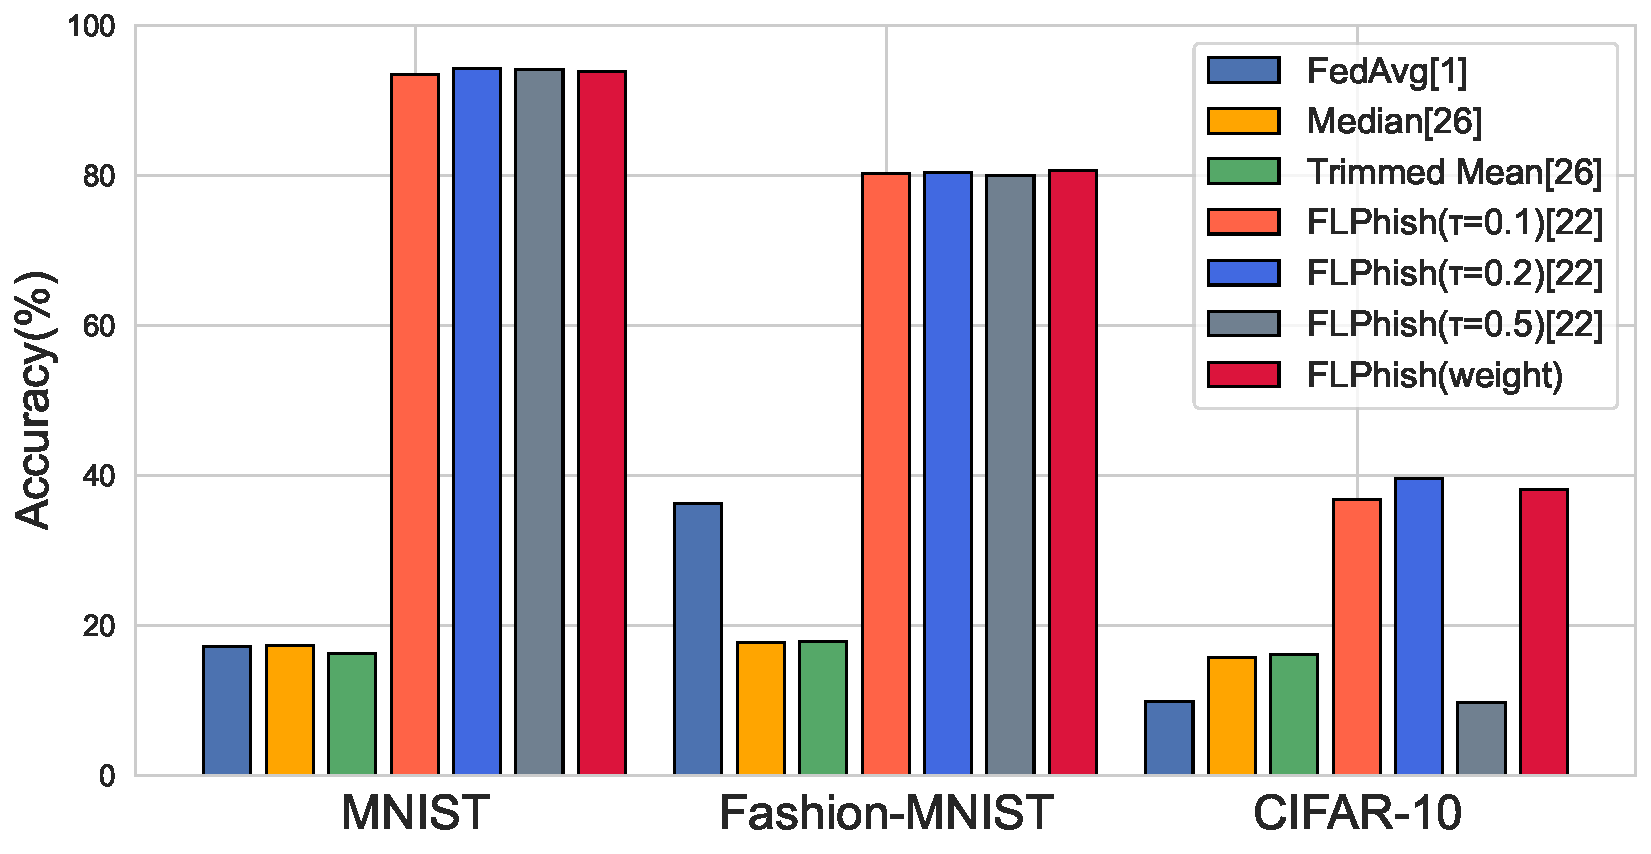
\includegraphics[width=0.48\textwidth]{figures/bar_byzantines_random_bar.pdf}}
    \subfloat[Byzantine Fraction 0.9 \& Imbalance Degree 0.2 \& Untargeted Attack]{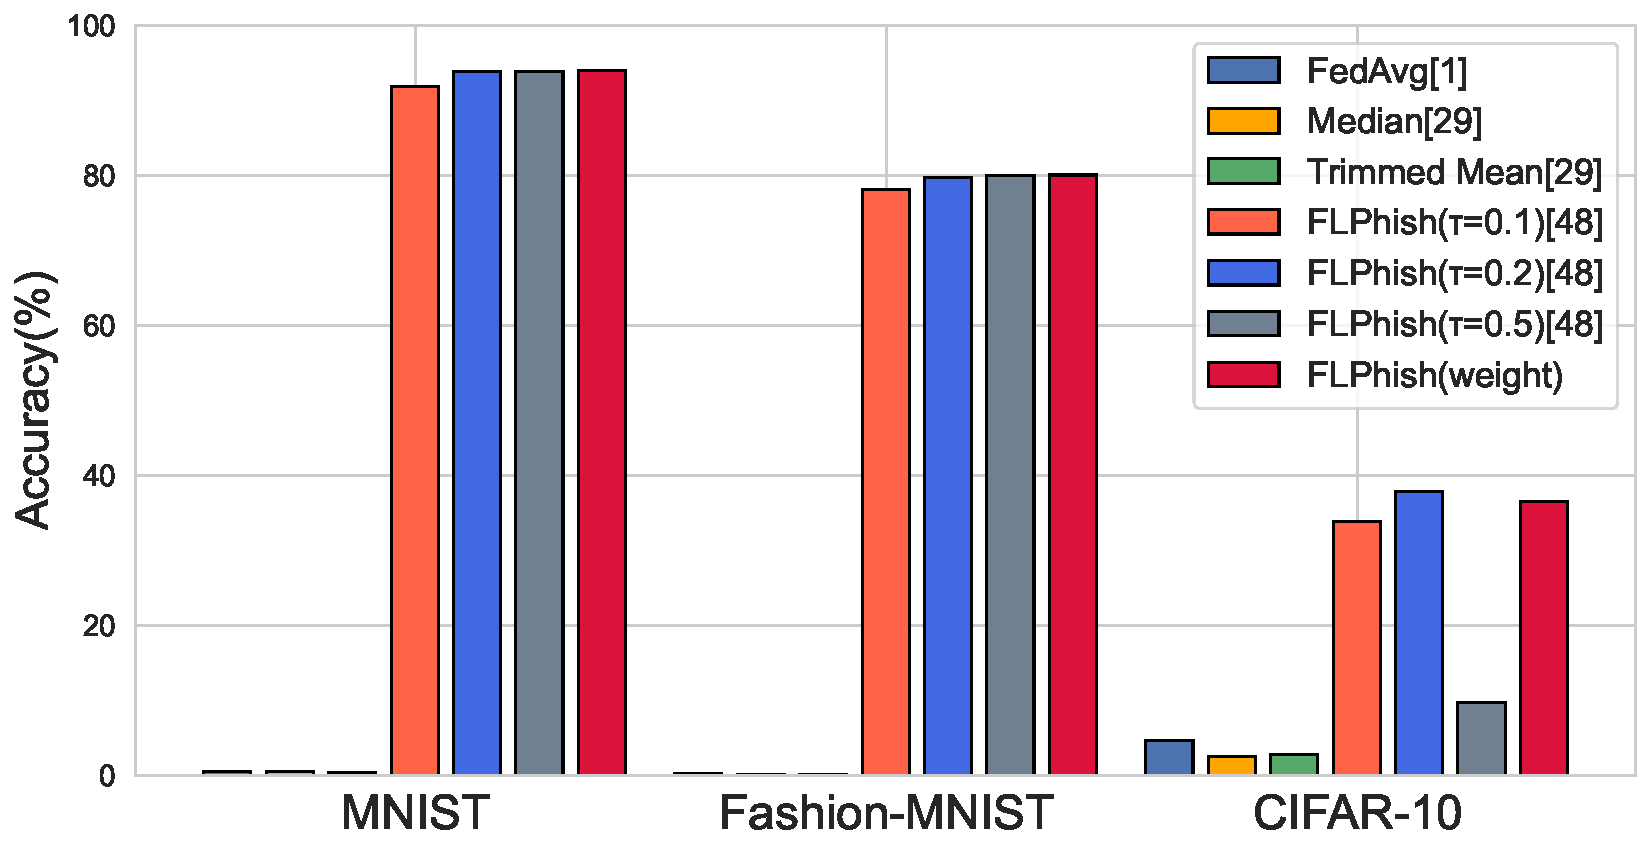
\includegraphics[width=0.48\textwidth]{figures/bar_byzantines_untargeted_bar.pdf}}
    \hfill
    \subfloat[Byzantine Fraction 0.5 \& Imbalance Degree 0.8 \& Random Attack]{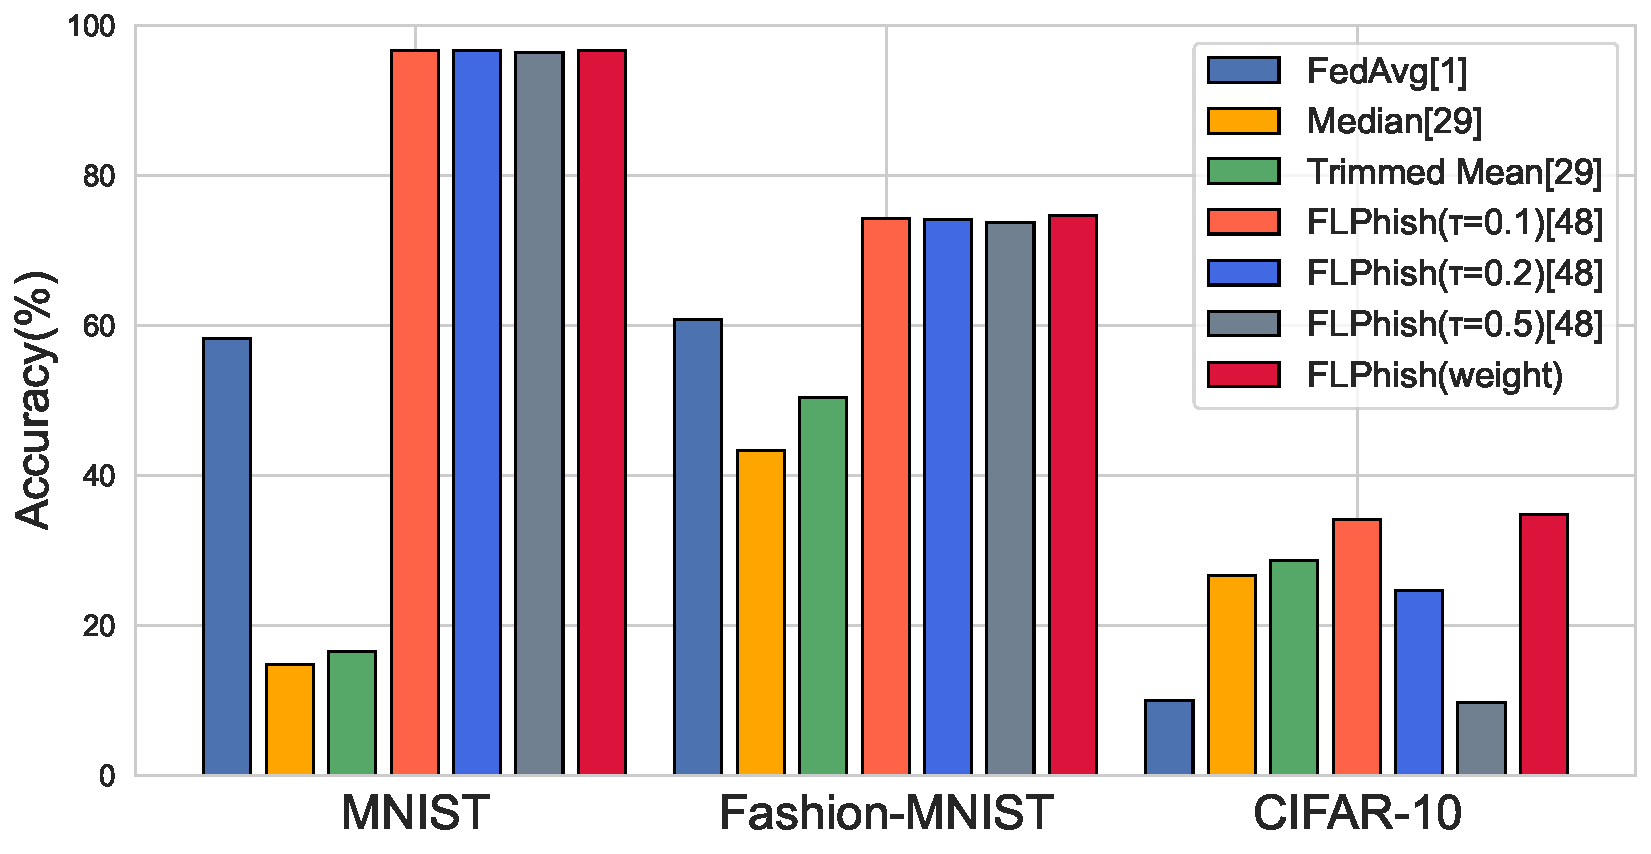
\includegraphics[width=0.48\textwidth]{figures/bar_imbalances_random_bar.pdf}}
    \subfloat[Byzantine Fraction 0.5 \& Imbalance Degree 0.8 \& Untargeted Attack]{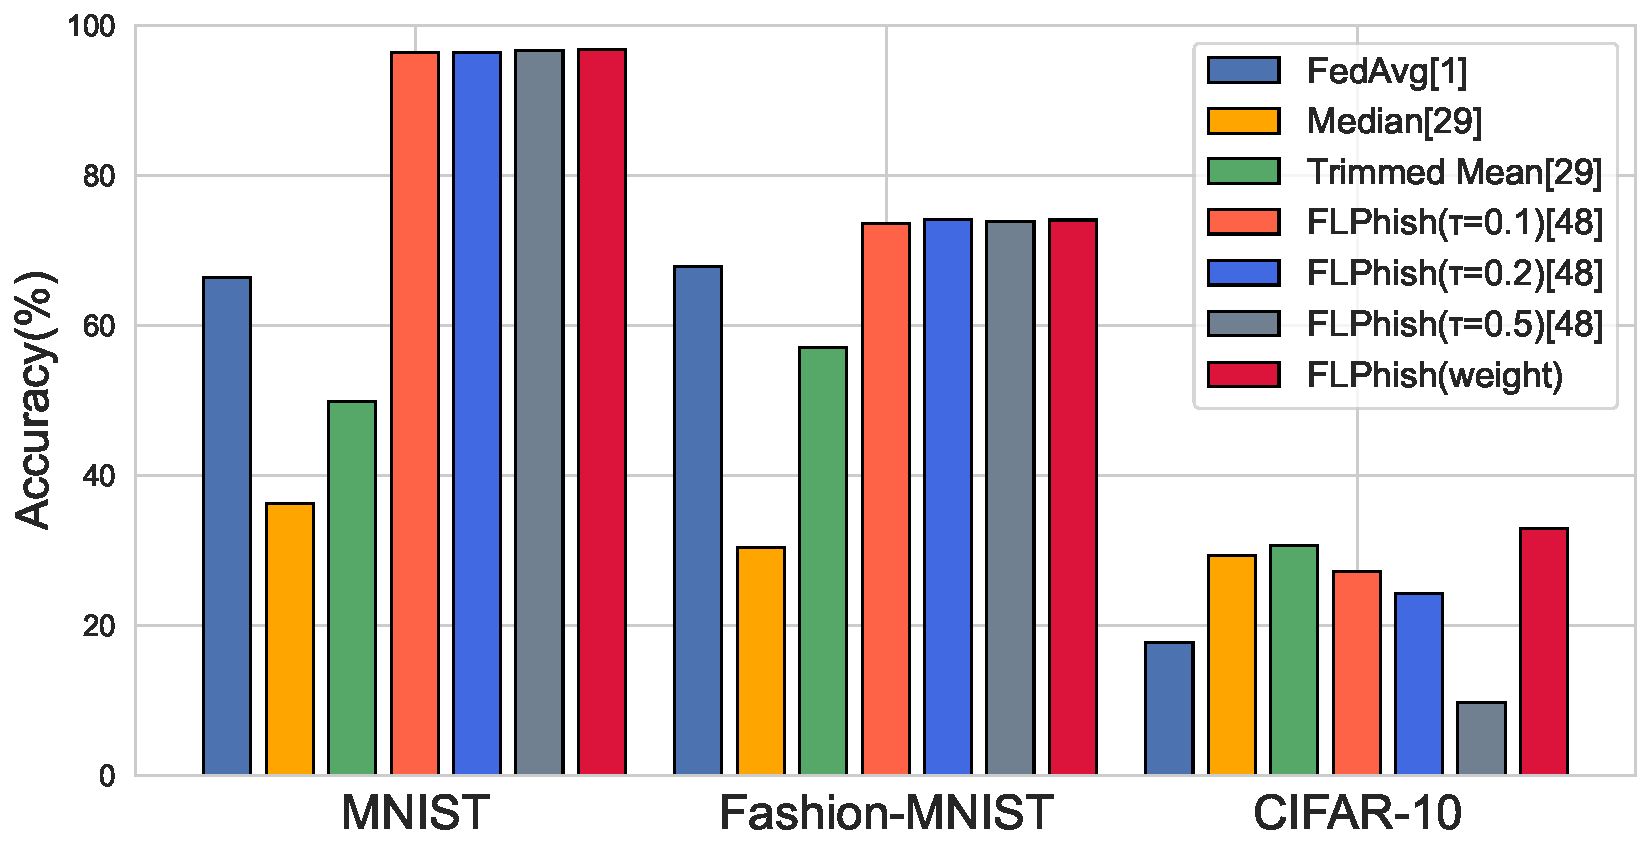
\includegraphics[width=0.48\textwidth]{figures/bar_imbalances_untargeted_bar.pdf}}
    \caption{Experiments results under different Byzantine fractions and different imbalance degrees.}
    \label{fig_exp_extreme}
  \end{figure*}



  \begin{figure*}[!htp]
    \centering
    \subfloat[MNIST]{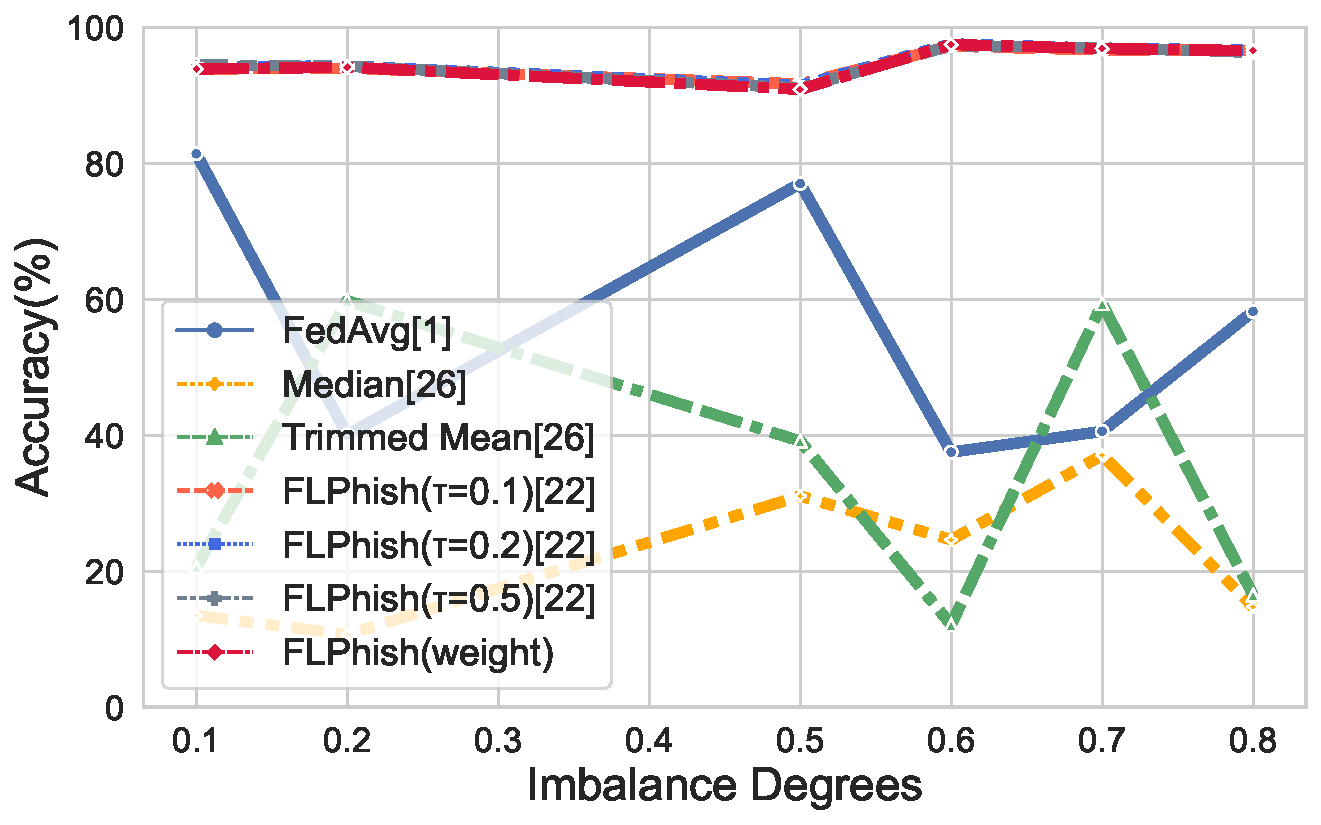
\includegraphics[width=0.325\textwidth]{figures/table_random_imbalances_MNIST.pdf}}
    \subfloat[Fashion-MNIST]{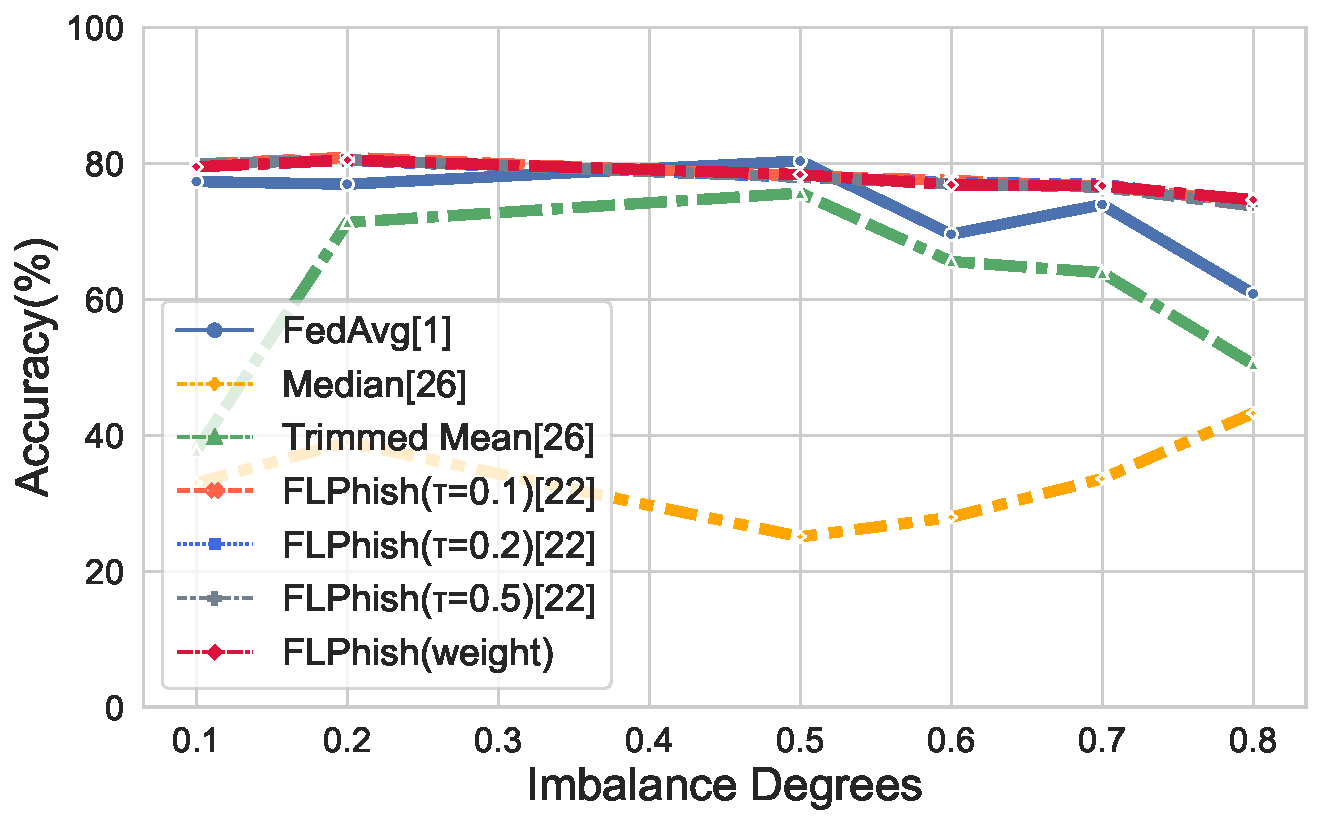
\includegraphics[width=0.325\textwidth]{figures/table_random_imbalances_Fashion-MNIST.pdf}}
    \subfloat[CIFAR-10]{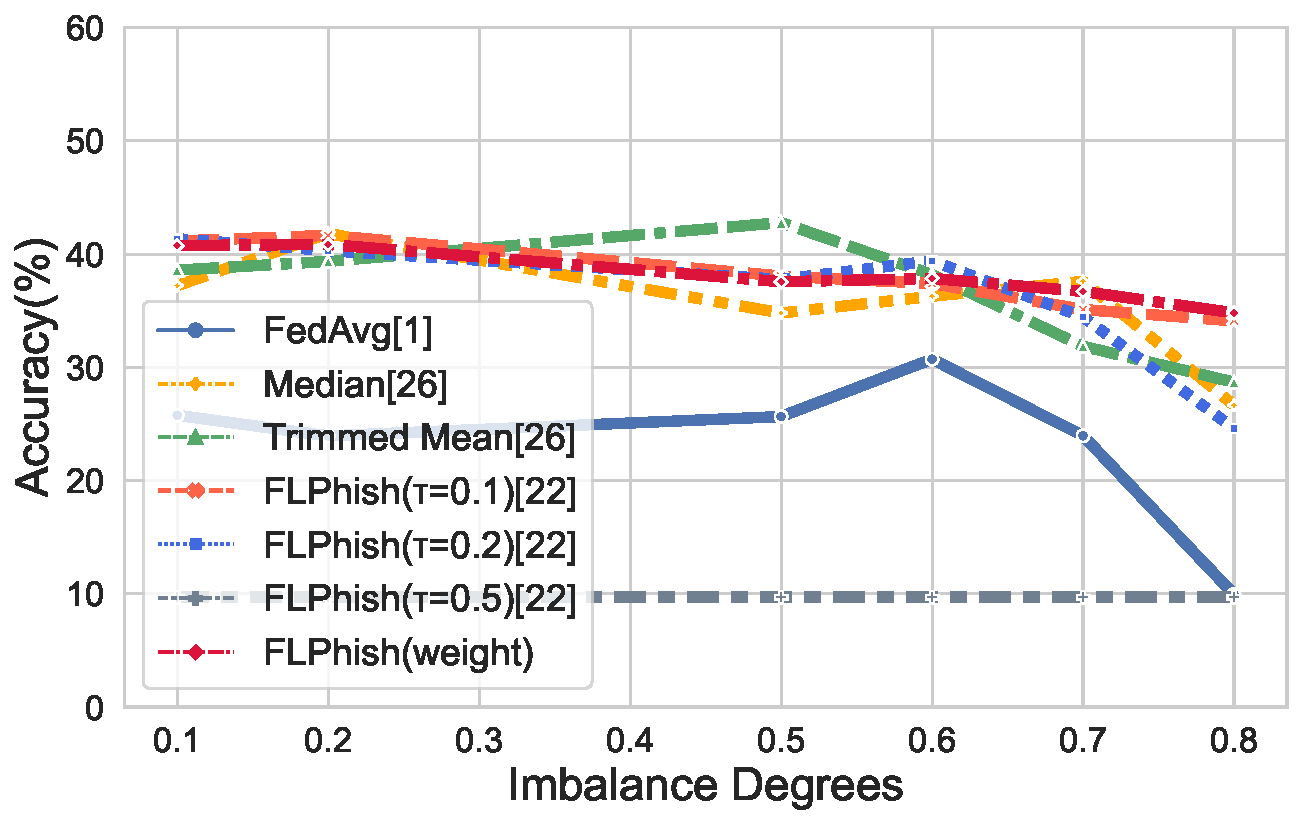
\includegraphics[width=0.325\textwidth]{figures/table_random_imbalances_Cifar-10.pdf}}
    \\
    \caption{Accuracy values on Different Imbalance Degrees under Random Attack.}
    \label{fig_table_imbalances_random}
  \end{figure*}

  \begin{figure*}[!htp]
    \centering
    \subfloat[MNIST]{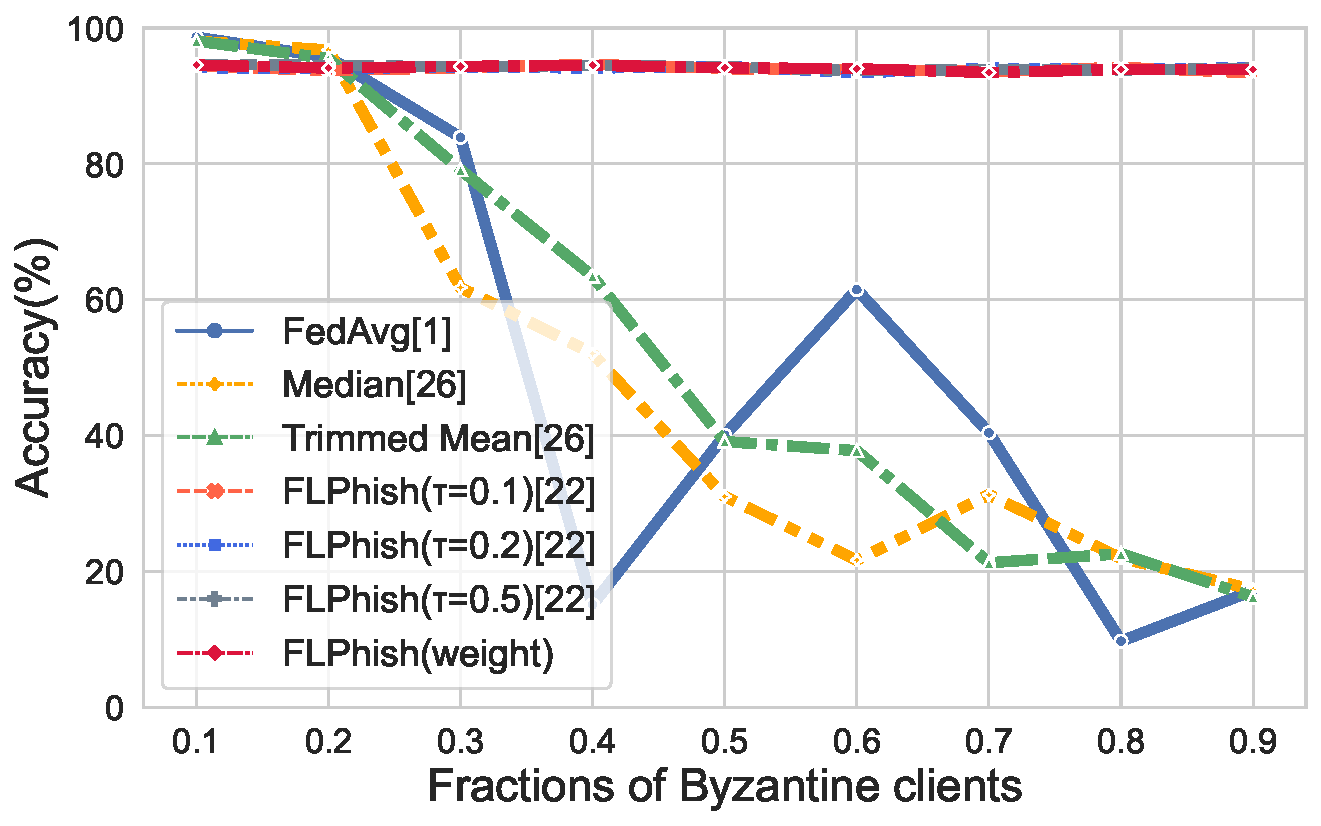
\includegraphics[width=0.325\textwidth]{figures/table_random_byzantines_MNIST.pdf}}
    \subfloat[Fashion-MNIST]{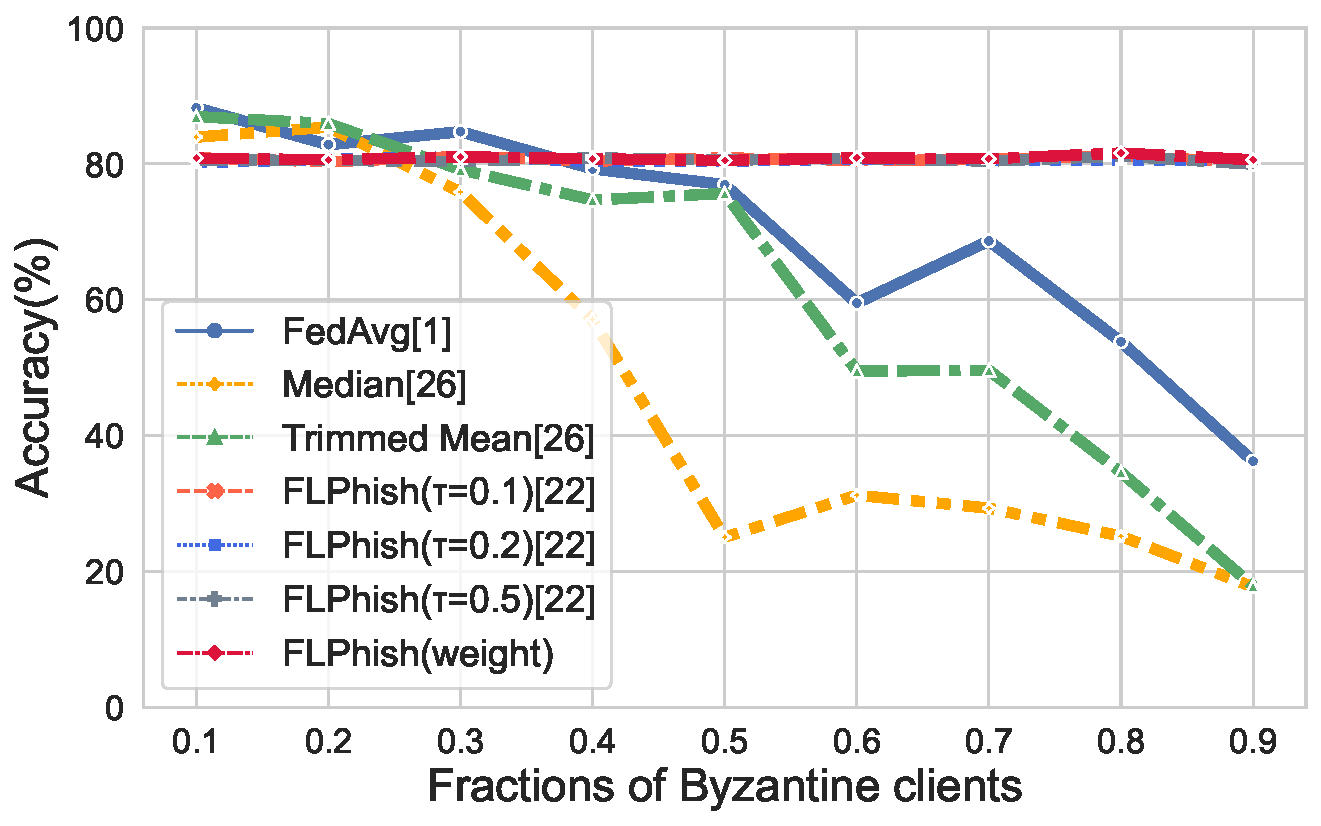
\includegraphics[width=0.325\textwidth]{figures/table_random_byzantines_Fashion-MNIST.pdf}}
    \subfloat[CIFAR-10]{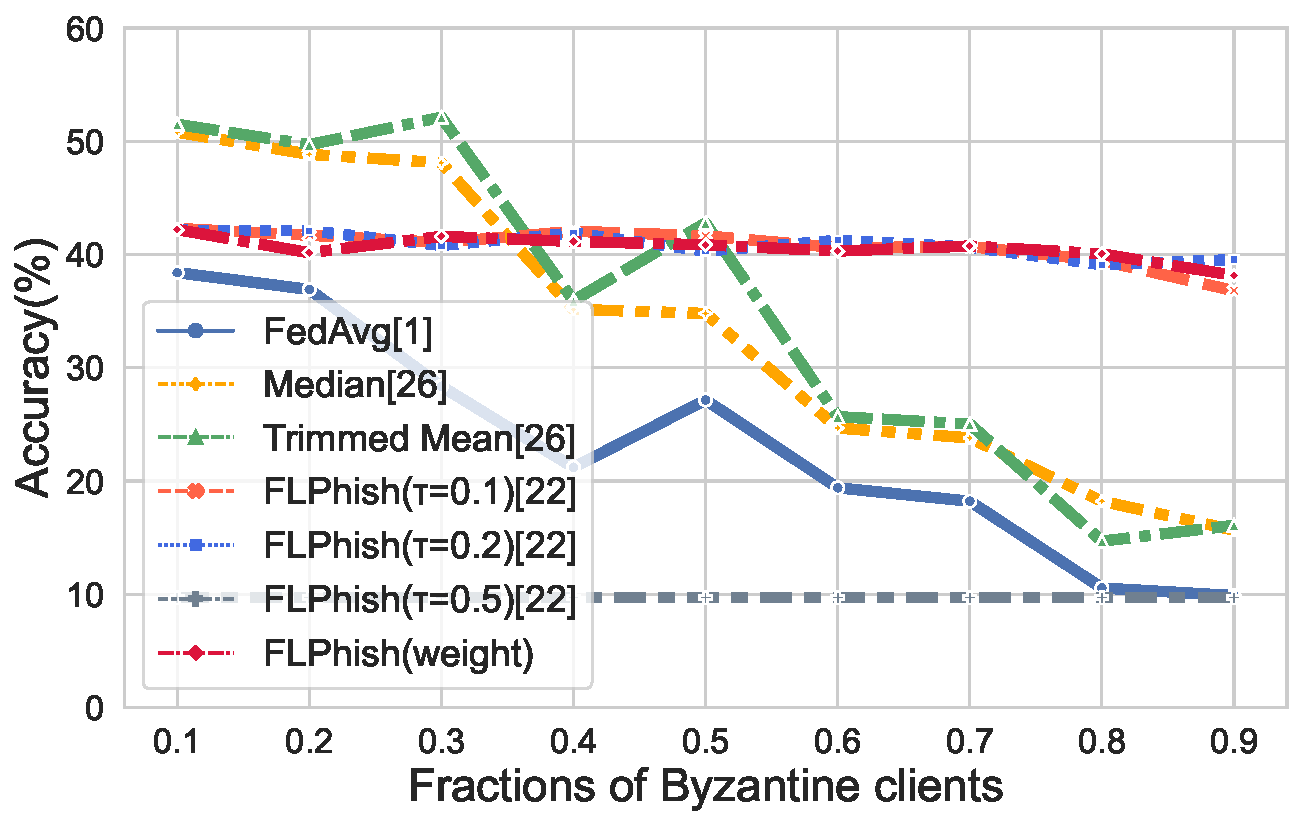
\includegraphics[width=0.325\textwidth]{figures/table_random_byzantines_Cifar-10.pdf}}
    \\
    \caption{Accuracy values on Different Byzantine Fractions under Random Attack.}
    \label{fig_table_byzantines_random}
  \end{figure*}


  \par Each client has 1,000 samples taken from the training dataset. Among the samples, 800 of them are used as training datasets, while another 200 are taken as test datasets. And the server has 10000 testing examples from the testing dataset. 
  \subsubsection{\textit{Evaluated Byzantine Attacks}} We evaluate our FLPhish(weight) against two Byzantine denial-of-service attacks mentioned in Section III.B:
  \begin{itemize}
    \item Untargeted Byzantine Attacks: For each Byzantine client, it mislabels the data $l$ to $(l-1)\ mod\ M$ to launch the attacks against FLPhish(weight). The attack is known as the Label-flipping attack. 
    \item Random Byzantine Attacks: For each Byzantine client, it mislabels the labels by returning a randomly chosen result.
    \end{itemize}

  
  \subsubsection{{\textit{Experiment Environment}}} We conduct all the experiments on a laptop with Intel(R) Core(TM) i7-11800H CPU 2.30GHz and an NVIDIA GeForce RTX 3060 GPU with the video memory of 6 GB. We implement all deep learning models using Keras\footnote{https://keras.io/}.



  \begin{figure*}[!htp]
    \centering
    \subfloat[MNIST]{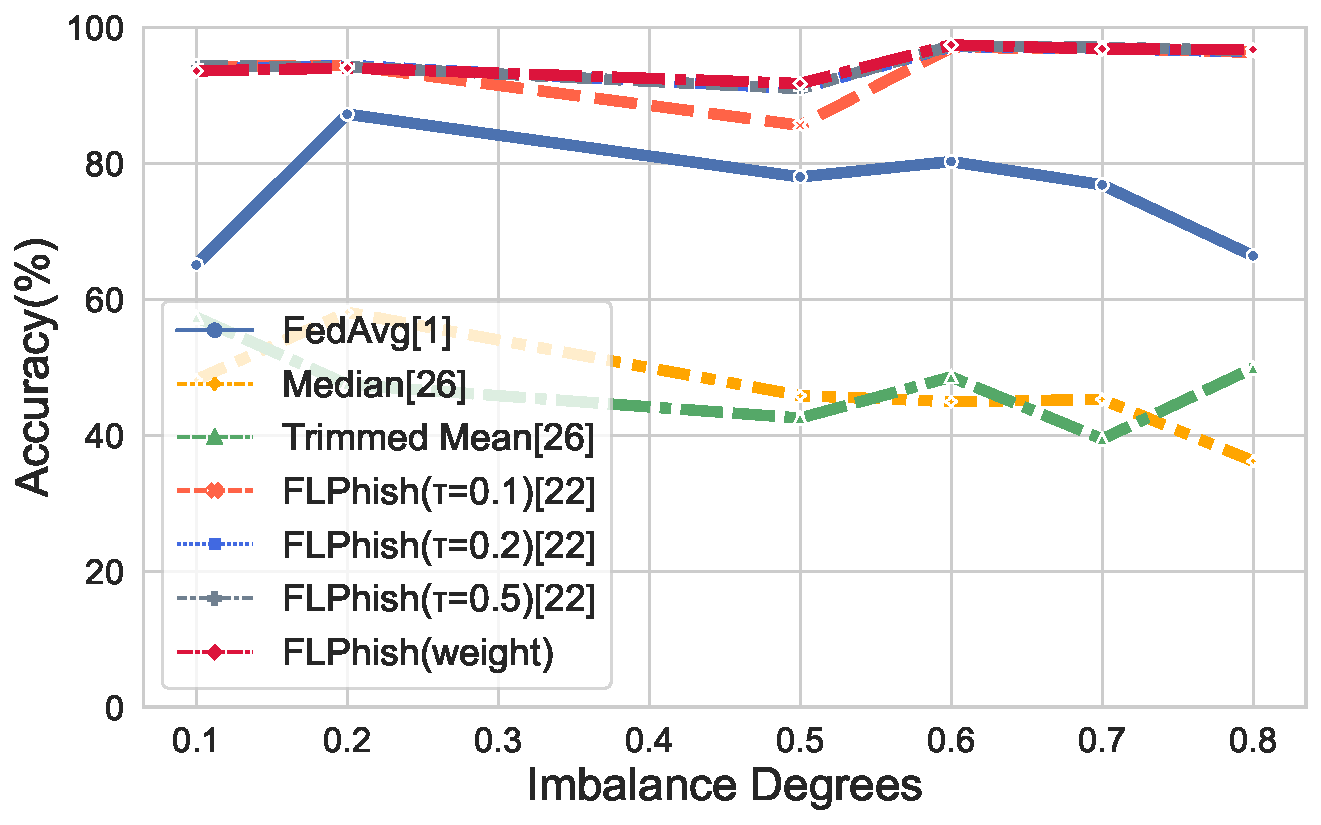
\includegraphics[width=0.325\textwidth]{figures/table_untargeted_imbalances_MNIST.pdf}}
    \subfloat[Fashion-MNIST]{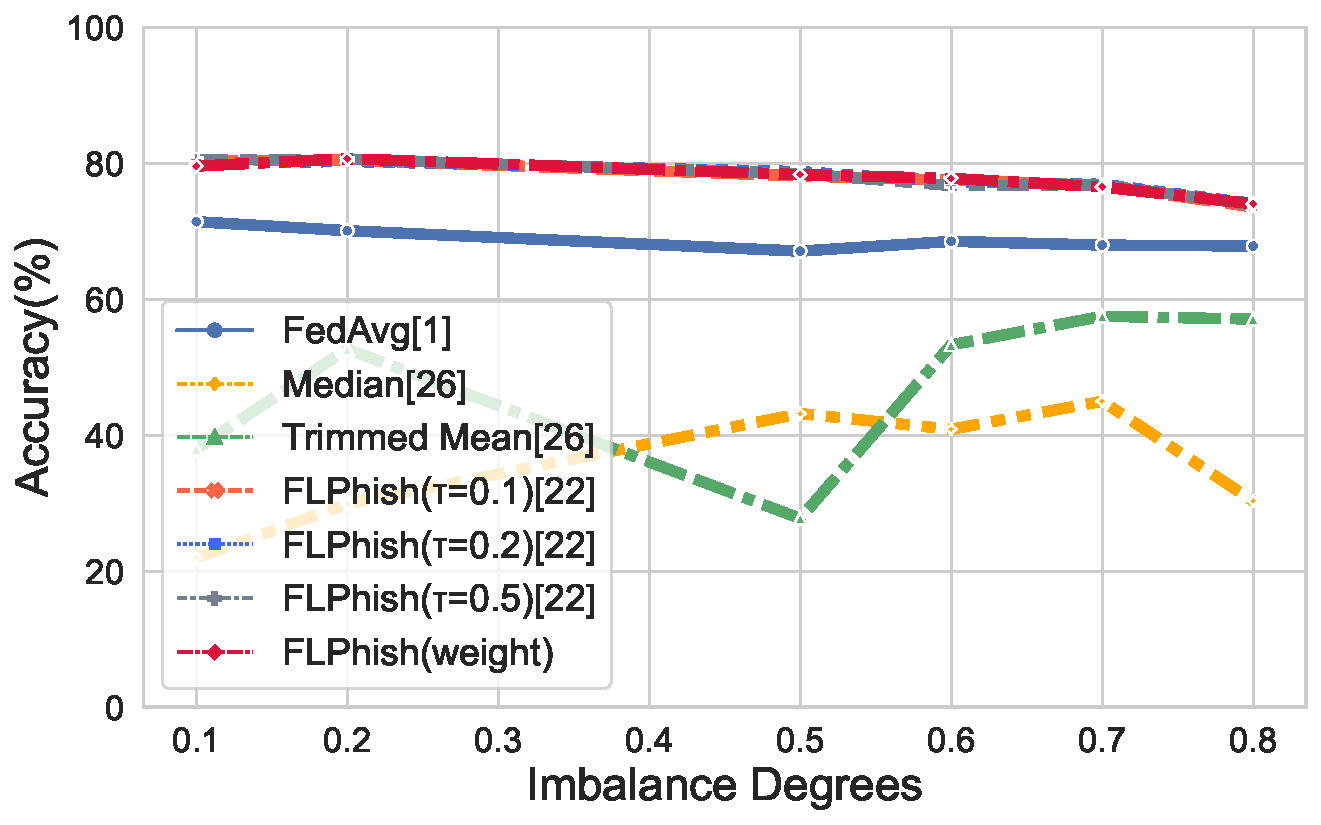
\includegraphics[width=0.325\textwidth]{figures/table_untargeted_imbalances_Fashion-MNIST.pdf}}
    \subfloat[CIFAR-10]{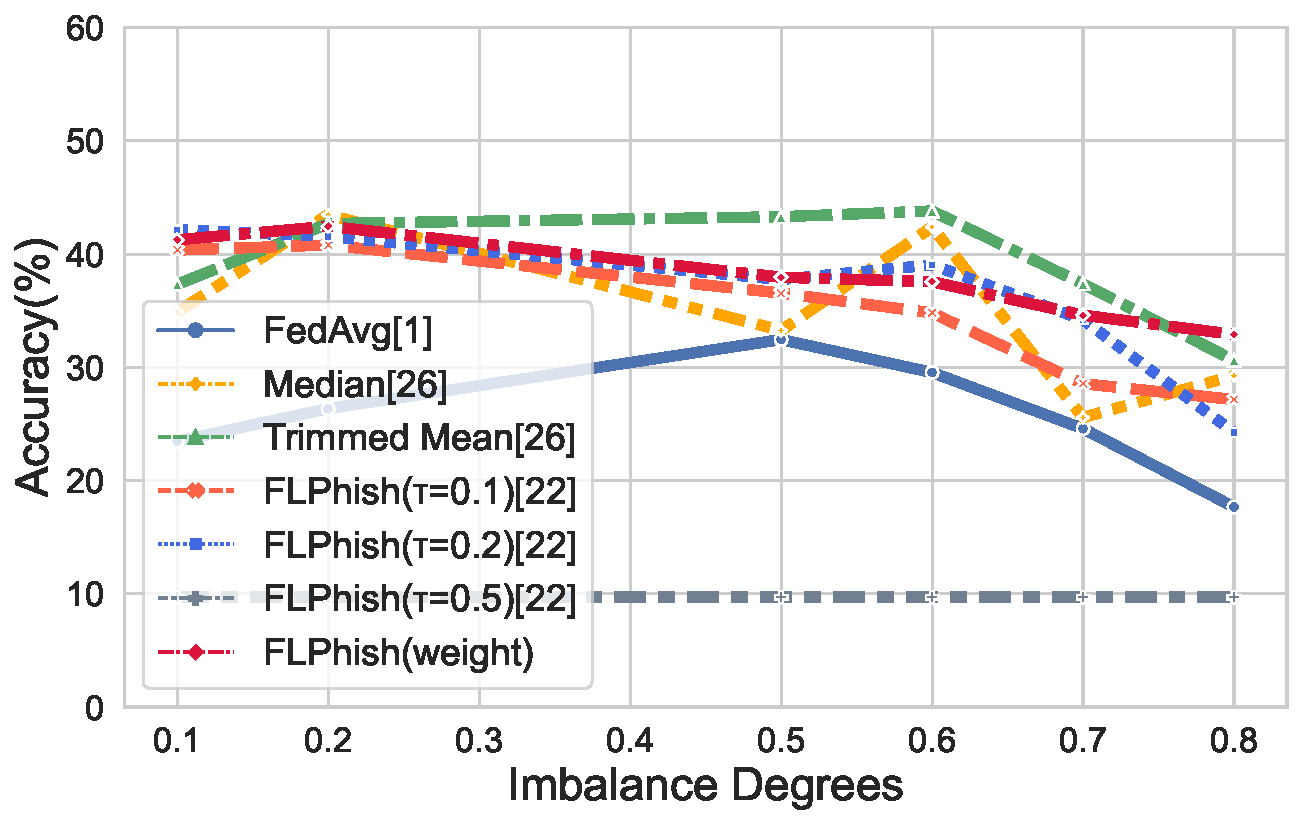
\includegraphics[width=0.325\textwidth]{figures/table_untargeted_imbalances_Cifar-10.pdf}}
    \\
    \caption{Accuracy values on Different Imbalance Degrees under Untargeted Attack.}
    \label{fig_table_imbalances_untargeted}
  \end{figure*}

  \begin{figure*}[!htp]
    \centering
    \subfloat[MNIST]{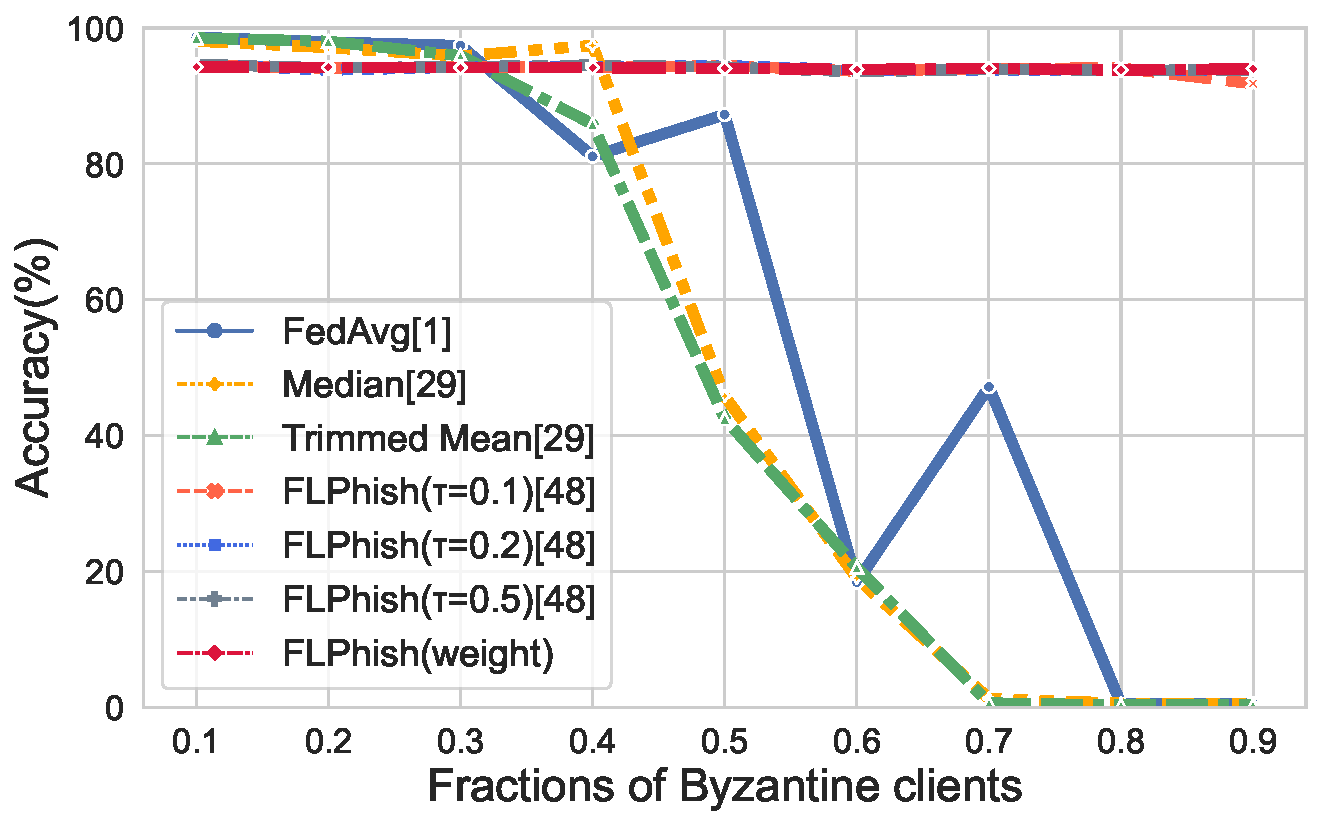
\includegraphics[width=0.325\textwidth]{figures/table_untargeted_byzantines_MNIST.pdf}}
    \subfloat[Fashion-MNIST]{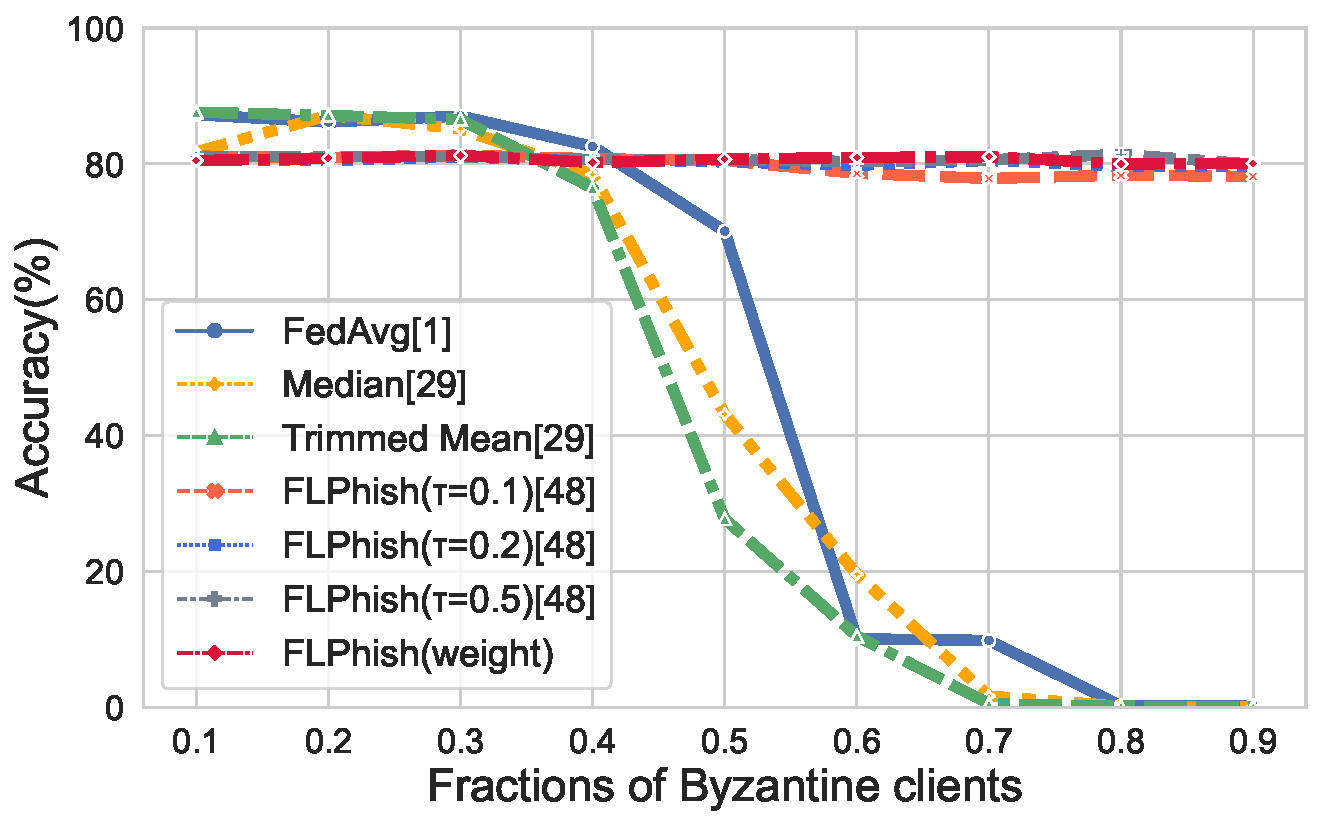
\includegraphics[width=0.325\textwidth]{figures/table_untargeted_byzantines_Fashion-MNIST.pdf}}
    \subfloat[CIFAR-10]{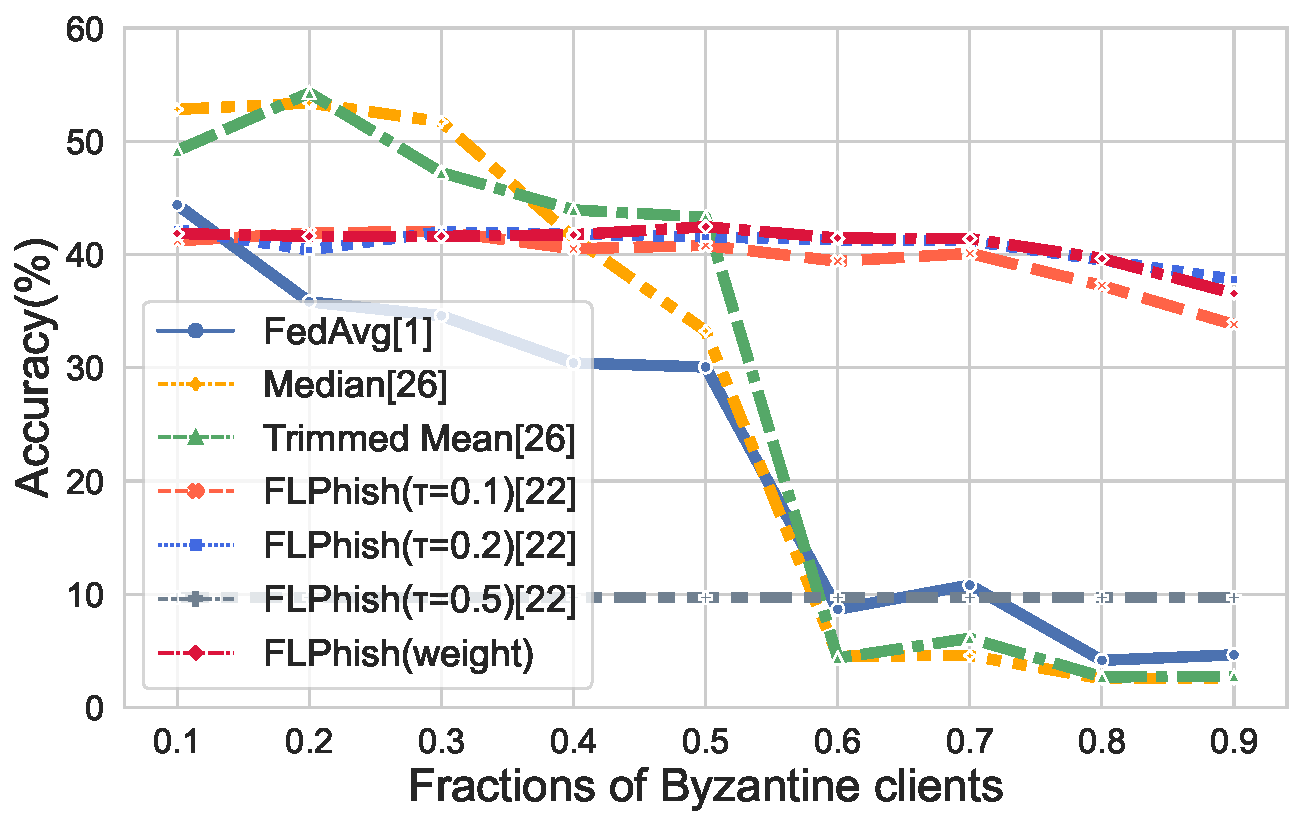
\includegraphics[width=0.325\textwidth]{figures/table_untargeted_byzantines_Cifar-10.pdf}}
    \\
    \caption{Accuracy values on Different Byzantine Fractions under Untargeted Attack.}
    \label{fig_table_byzantines_untargeted}
  \end{figure*}




  \subsection{Performance Comparison under Random Attacks}
  From Fig. \ref{fig_exp_extreme}-\ref{fig_table_byzantines_random}, we can see that random Byzantine attacks have poor performance against FLPhish(weight) and FLPhish($\tau$=0.1, 0.2). We refer from the result that a random Byzantine attack has a drawback that it can not gather its influence at one data point as untargeted Byzantine attackers do. Meanwhile, we can see that it has good results in attacking FLPhish($\tau$=0.5) in the CIFAR-10 dataset. From Fig. \ref{fig_exp_reputation}, we can see that the reputation of benign clients in CIFAR-10 experiments rapidly falls under the threshold of 0.5 due to the complexity of the tasks. With the increase of imbalance degree value $q$, the reputation of the benign clients falls more rapidly in the experiments of the CIFAR-10 dataset than in the experiments of the MNIST and the Fashion-MNIST dataset. As benign clients' reputations in the experiments of the CIFAR-10 dataset become under the threshold $\tau$ of 0.5, they are identified as malicious Byzantine clients as well. As many benign clients are falsely identified as Byzantine attackers, the FL server lacks enough trusted FL clients to assist the aggregation, therefore causing a bad performance of FLPhish($\tau$=0.5). Meanwhile, we can see that FLPhish($\tau$=0.1), FLPhish($\tau$=0.2), and FLPhish(weight) stood still against the random Byzantine attacks. The results indicate that the value of the threshold $\tau$ should be considered carefully in the application in some complex tasks.








  \subsection{{Performance Comparison under Untargeted Attacks}} We further evaluate FLPhish(weight) towards untargeted Byzantine attacks in EFL.
  

  
    \subsubsection{\ul{Performance Comparison with Different Distributions}} We test our FLPhish(weight) in an experiment environment with a fixed Byzantine client fraction of 0.5 and a variable distribution imbalance value $q$ across tests. The experiment results are shown in Fig. \ref{fig_table_imbalances_untargeted}. We can see that both FLPhish($\tau$=0.1,0.2,0.5) and FLPhish(weight) outperform other schemes. When the imbalance degree $q$ reaches 0.8, the distribution of data becomes very non-IID. In this situation, the FLPhish($\tau$=0.5)'s performance progressively deteriorates. When confronted with a distribution with an imbalance degree of $q=0.8$, each client performs poorly, resulting in a loss of reputation. The accuracy of the global model declines sharply as the degree of imbalance rises. Throughout the learning phase, the accuracy of the global model under FLPhish($\tau$=0.5) remains at 0.1. It means that FLPhish($\tau$=0.5) considers all clients to be Byzantine, thus invalidating the aggregation process. As can be seen, the FLPhish($\tau$=0.2) outperforms the FLPhish($\tau$=0.1,0.5). To avoid a high false-negative rate, the threshold $\tau$ of FLPhish($\tau$) should be set to a lower value when the distribution becomes non-IID. It should be set to 0.2 in the MNIST experiment. Meanwhile, FLPhish(weight) maintains its performance under varying degrees of imbalance.
    


    
    \subsubsection{\ul{Performance Comparison with Different Fractions of Byzantine Clients}} Different fractions of Byzantine clients are taken into account as well. Figure. \ref{fig_table_byzantines_untargeted} shows that the accuracy for FedAvg, Median and Trimmed Mean begins to fall rapidly when the Byzantine portion reaches nearly 50\%. Furthermore, FedAvg, Median, and Trimmed Mean perform extremely invalidly (the accuracy falls below 1\%) when encountered with high fractions of Byzantine attackers. In comparison, FLPhish($\tau$) and FLPhish(weight)'s performance under various thresholds maintain a high level of performance as the portion grows. Both FLPhish($\tau$) and FLPhish(weight) effectively detect Byzantine clients and accurately discard them from the aggregation process. The global model can be successfully trained without the involvement of Byzantine clients during the aggregation procedures. Furthermore, the data show that FLPhish($\tau$=0.1) performs worse than the other two. This is since the threshold=0.1 is far too low to adequately detect Byzantine clients. Though the Byzantine attackers try to make the right predictions of the public dataset and then send the opposite wrong predictions to the FL server. But they also make wrong predictions first and coincidentally transfer the opposite right predictions to the FL server. Thus the reputation values of some Byzantine clients, in particular, can exceed 0.1. It indicates that if the threshold is not well set, Byzantine clients can avoid being detected by FLPhish($\tau$). As the fractions of Byzantine clients go over the threshold of 50\%, the harm brought by untargeted Byzantine attacks increase rapidly for they outnumber the fractions of the benign clients. In the meantime, FLPhish(weight) shows stable performance whenever the fractions of Byzantine clients are.

    \subsection{{Experiment Result Analysis}} Our experiment results demonstrate that both FLPhish($\tau$) and FLPhish(weight) outperform FedAvg, Median \cite{ref_13_defense} and Trimmed Mean \cite{ref_13_defense} on defending against Byzantine attacks in FL. The results also show that the threshold setup has a significant impact on the performance of the FLPhish($\tau$). Only when the managers of FL servers have complete knowledge of FL clients (the imbalance degree of each client), can they accurately set the value of the threshold suitably. However, it is not feasible due to the privacy concern of FL. FLPhish(weight), on the other hand, remains constant regardless of the circumstances. FLPhish(weight) can let clients with higher performance have a stronger influence on the aggregation process by using the reputation value as the weight. To summarize, FLPhish(weight) is a better and more stable aggregation technique than FLPhish(weight) and demonstrates to be a more practical Byzantine defense framework.


\section{Conclusion}
In this paper, we have designed an FL architecture, Ensemble Federated Learning (called EFL), which allows knowledge transfer between the FL server and FL clients via an unlabeled dataset and the FL clients' predictions of it. We have crafted the FLPhish technique to make EFL resistant to Byzantine attacks by using a labeled dataset as `bait' to detect malicious Byzantine clients. Furthermore, we have proposed a reputation technique based on Bayesian inference to determine a client's level of trust. We have proved the security of the FLPhish scheme against backdoor attacks. Finally, we have tested our suggested FLPhish in a variety of scenarios. The results of the experiment demonstrate the comparable performance of FLPhish in terms of accuracy and robustness under Byzantine attacks in FL. 
\par Our future work will focus on evaluating FLPhish against more advanced Byzantine attacks and improving the FLPhish scheme's efficiency.




\bibliography{IEEEabbrv}
\bibliographystyle{IEEEtran}


\end{document}


